\documentclass[12pt,a4paper]{report}
%\documentclass[12pt,a4paper,twoside,openright]{book}
\usepackage[utf8]{inputenc}
\usepackage[english]{babel}
\usepackage[T1]{fontenc}
\usepackage{latexsym}
\usepackage[final]{graphicx} %draft % To include graphics
%\usepackage{epsfig}
\usepackage{amsmath,amssymb,amsthm}
\usepackage[none]{hyphenat} 
\usepackage[small,bf]{caption}
\usepackage{float} % parametro H in figure : posizionamento esattamente li
\usepackage{verbatim}
\usepackage{booktabs}
\usepackage{enumerate} %lettere o altro negli indici
\usepackage{hyperref} % prima di algorithm
\usepackage{algorithmic} %float con un algoritmo
\usepackage[ruled]{algorithm} %[boxed]
\usepackage{subfig}    % + figure in un float figure
\usepackage{datetime}
%\usepackage{xcolor} va in conflitto con il paccketto color se c'è l'opzione [usenames]
\usepackage[usenames, dvipsnames]{color} %testo colorato
\usepackage{tikz}
\usepackage[]{fullpage}
\usepackage{fancybox}
\usepackage{rotating}
\usepackage{supertabular}
\usepackage{appendix}
\usepackage{dcolumn} %per usare direttamente il punto al posto di & nei decimali
\usepackage{listings}
\usepackage{textcomp} % per upquote=true di listings
\usepackage{epstopdf} % per importare gli eps con \includegraphics
\usepackage{numprint}
%\usepackage{indentfirst}
%\usepackage[Lenny]{fncychap} % [Sonny[Lenny] 
\usepackage{threeparttable} %gestire le note sotto le tabelle float
\usepackage{relsize} %dimensioni relative più grandi o piccole

%definisce il comando \symbolfootnote per mettere le note con simbolo. che nelle equazioni altrimenti c'è casino
\long\def\symbolfootnote[#1]#2{\begingroup%
\def\thefootnote{\fnsymbol{footnote}}\footnote[#1]{#2}\endgroup}
%use \symbolfootnote[1-2-3-4...-9]{footnote}

% LINKS
%http://www.kronto.org/thesis/tips/index.html

% COMANDO PER PRIMA REVISIONE

\newcommand{\rev}[1]{\textcolor{Cerulean}{#1}}

\captionsetup[lstlisting]{skip=10pt}
\lstset{ %
language=Matlab,                % choose the language of the code
basicstyle=\footnotesize,       % the size of the fonts that are used for the code
numbers=left,                   % where to put the line-numbers
numberstyle=\footnotesize,      % the size of the fonts that are used for the line-numbers
stepnumber=1,                   % the step between two line-numbers. If it's 1 each line will be numbered
numbersep=5pt,                  % how far the line-numbers are from the code
backgroundcolor=\color{white},  % choose the background color. You must add \usepackage{color}
showspaces=false,               % show spaces adding particular underscores
showstringspaces=false,         % underline spaces within strings
showtabs=false,                 % show tabs within strings adding particular underscores
frame=single,	                % adds a frame around the code
tabsize=2,	                % sets default tabsize to 2 spaces
captionpos=t,                   % sets the caption-position to bottom
breaklines=true,                % sets automatic line breaking
breakatwhitespace=false,        % sets if automatic breaks should only happen at whitespace
title=\lstname,                 % show the filename of files included with \lstinputlisting; also try caption instead of title
escapeinside={\%*}{*)}          % if you want to add a comment within your code
}

\DeclareMathOperator*{\argmax}{arg\,max}

% il compilatore converte gli eps di matlab in pdf e poi da quelli importa le immagini
% se trova il pdf prima usa quello per cui le modificihe all'eps vengono ignorate
% è pertanto necessario caricare prima l'eps per produrre il nuovo pdf da importare
\DeclareGraphicsExtensions{.eps,.pdf,.png,.jpg}

\definecolor{listinggray}{gray}{0.9} 
\definecolor{lbcolor}{rgb}{0.95,0.95,0.95} 

\lstset{
%	backgroundcolor=\color{lbcolor},
	tabsize=4,
	rulecolor=,
        basicstyle=\scriptsize,
        upquote=true,
        aboveskip={1.5\baselineskip},
        columns=fixed,
        showstringspaces=false,
        extendedchars=true,
        breaklines=true,
        prebreak = \raisebox{0ex}[0ex][0ex]{\ensuremath{\hookleftarrow}},
        frame=single,
        showtabs=false,
        showspaces=false,
        showstringspaces=false,
        identifierstyle=\ttfamily,
        keywordstyle=\color[rgb]{0,0,1},
        commentstyle=\color[rgb]{0.133,0.545,0.133},
        stringstyle=\color[rgb]{0.627,0.126,0.941},
        extendedchars=true,
        inputencoding=utf8,
}


\usetikzlibrary{arrows}
\usetikzlibrary{snakes}
%\pagestyle{headings} % {headings,plain ,empty} richiamato automaticamente da \usepackage[headings]{fullpage}

%con la classe book+openright lascio una pagina bianca a fine capitolo e dopo il titolo se necessario, con empty page queste pagine non sono numerate e non hanno stile
\usepackage{emptypage}

%\usepackage[all]{hypcap}

\usepackage{fancyhdr}

\newcommand{\pc}{p_{\epsilon}}
\renewcommand{\appendixname}{}
\renewcommand{\appendixtocname}{Appendices}
\setcounter{tocdepth}{3}

\frenchspacing
\linespread{1.3}
\DeclareGraphicsRule{.eps,.ps,.png}{bmp}{.bb}{} % formati utilizzabili con ordine di preferenza 
                                                % cosi non devo indicare le estensioni
\newcommand{\HRule}{\rule{\linewidth}{0.5mm}}

\newcommand{\algname}[1]{\ensuremath{\mbox{\sc #1}}}

\renewcommand{\algorithmicrequire}{\textbf{Input:}}
\renewcommand{\algorithmicensure}{\textbf{Output:}}
\renewcommand{\algorithmiccomment}[1]{// #1}

\algsetup{indent=2em} 

\hypersetup{
    bookmarks=true,         % show bookmarks bar?
    unicode=false,          % non-Latin characters in Acrobat’s bookmarks
    pdftoolbar=true,        % show Acrobat’s toolbar?
    pdfmenubar=true,        % show Acrobat’s menu?
    pdffitwindow=false,     % window fit to page when opened
    pdfstartview={FitH},    % fits the width of the page to the window
    pdftitle={Batch Size Estimate},    % title
    pdfauthor={Marco Bettiol},     % author
    pdfsubject={Subject},   % subject of the document
    pdfcreator={Creator},   % creator of the document
    pdfproducer={Producer}, % producer of the document
    pdfkeywords={batch resoluzion algorithms, wireless sensor networks}, % list of keywords
    pdfnewwindow=true,      % links in new window
    colorlinks=true,       % false: boxed links; true: colored links
    linkcolor=black,          % color of internal links
    citecolor=black,        % color of links to bibliography
    filecolor=black,      % color of file links
    urlcolor=black           % color of external links
}


%per impaginare con giustifica sx-dx
  \tolerance 1414
  \hbadness 1414
  \emergencystretch 1.5em
  \hfuzz 0.3pt
  \widowpenalty=10000
  \vfuzz \hfuzz
  \raggedbottom

\title{Batch Size Estimate}
\author{Marco Bettiol}

\begin{document}

% !TEX root = tesi.tex
\begin{titlepage}

		\thispagestyle{empty}
    \begin{figure}
    \centering
      \subfloat{
\includegraphics[scale=1]{immagini/logo_unipd_black}}\quad     \subfloat{
\includegraphics[scale=1.3]{immagini/DEIlogoFULL}}
    \end{figure}
    
    \vskip 3cm{
    \begin{center}\sc
        UNIVERSITY OF PADUA\\
        DEPARTMENT OF INFORMATION ENGINEERING\\
        MASTER DEGREE IN COMPUTER ENGINEERING\end{center}
		}
		
		\vskip1.2cm\begin{center}
      \rm\large\uppercase\expandafter{A.A. 2009/2010\\}
 \end{center}
    	
    \vskip 2.5cm\begin{center}
    \HRule \\[0.4cm]\LARGE\expandafter{BATCH SIZE ESTIMATE}
    \HRule \\[0.4cm]
    \end{center}
    
    \begin{flushright}\vskip4.0cm 
    \begin{tabular}{rl}
            \rm\large \uppercase{Supervisor:} &\emph{Prof. Andrea Zanella}\\
	   \rm\large \uppercase{Student:} &\emph{Marco Bettiol} \\
		\end{tabular}
     \end{flushright}
    \vfill
          \begin{center}
                  \vskip1.0cm 
                  Last Update: \today  \hspace{1mm } \currenttime
           \end{center}
    
\end{titlepage}

\newpage
%%pagina vuota
%\clearpage\null\thispagestyle{empty}\clearpage

%\setcounter{page}{1}

%% DEDICATION
\begin{comment}
\begin{flushright}
\null\vspace{\stretch{5}}
\emph{\large Ai miei genitori}
\vspace{\stretch{1}}\null
\end{flushright}
\begin{abstract}
This thesis
\end{abstract}
\end{comment}


\tableofcontents
\listoffigures
\listoftables
%\listofalgorithms

\chapter{Introduction}

Generally speaking a set of actors contending for a common resource define a \emph{conflicting set}. As always, limited resources require policies to access them in an efficient and hopefully fair way. When the system is distributed, and this is our case, resource access can be assimilated to a coordination problem.\\ 
\rev{In our scenario the contended resource is the physical transmission medium that is shared by several stations.}\\ \rev{At the beginning of wired computer networks, multiple access control (MAC) was a big issue for efficient communications. The introduction of packet buffered switches  in LANs reduced the conflicting set to \textcolor{red}{only two stations (NOTA: \emph{why??} RISPOSTA:perchè un cavo ha solo 2 estremità e nelle reti switched ogni porta appartiene ad un solo dominio di collisione (non è un hub ma uno switch))}  simplifying  the original problem. Switched networks, in fact, split large collision domains into smaller pieces thus realizing ring, star or mesh structures.\\ 
In a wireless context the problem can not be easily avoided, due to the broadcast nature of the wireless medium.\\  
}

Nowadays wireless connectivity in pervasive computing has ephemeral character and can be used for creating ad-hoc networks, sensor networks, connections with RFID (Radio Frequency Identification) tags etc. The communication tasks in such wireless networks often involve an inquiry over a shared channel, which can be invoked for discovery of neighboring devices in ad-hoc networks, counting the number of RFID tags that have a certain property, estimating the mean value contained in a group of sensors etc. Such an inquiry solicits replies from possibly large number of terminals.\\

In particular we analyze the scenario where a reader broadcasts a query to the in-range nodes. Once the request is received, devices with data of interest are all concerned in transmitting the information back to the inquirer as soon as possible and, due to the shared nature of the communication medium,  while collision problems come in: only one successful transmission at time can be accomplished, concurrent transmissions result in destructive interference with inefficient waste of energy/time. This data traffic shows a bursty nature which is the worst case for all shared medium scenarios.\\

This problem is referred in literature with different names: \emph{Batch/Conflict Resolution Problem}, \emph{Reader Collision Problem}, \emph{Object Identification Problem}.\\
Algorithms trying to solve this problem efficiently  are called \emph{Batch Resolution Algorithms} (BRA) or  \emph{Collision Resolution Algorithms} (CRA).\\ 

In our terminology a query determines a subset of nodes which have to reply with one (and only one) message: this set of nodes constitutes the \emph{batch}. The size of the batch can be known in advance, in lucky and optimistic scenarios, or \rev{it} can change in time.

Since each node has exactly one message to deliver, the problem of obtaining all the messages or counting the number of nodes involved by the resolution process is exactly the same.

\rev{
Instead the problem differs when we are not interested in the exact number of nodes but rather we aim at an estimate of the actual batch size, as accurate as possible.}

\rev{
The knowledge of the batch size $n$ is an important factor for parameters' optimization in order to improve the resolution efficiency  through the minimization of the time taken by the process.\\}

\section{Model}

We consider the following standard model of a multiple access channel. A large number of geographically distributed nodes communicate through a common radio channel. Any node generates a packet to be transmitted on the channel. Transmissions start at integer multiples of  time unit and last one unit of time called \emph{slot}.\\

\rev{
In \emph{pure-slotted} systems some form of synchronization among nodes is required to inform the nodes about the beginning of slots (or at least the beginning of a cycle of slots). Nodes can start a transmission only at the beginning of the slot, otherwise they will stay quiet until the next slot to come.\\}

\rev{
In \emph{CSMA} networks each node is able to determine the beginning of a new slot by sensing the energy on the channel: when the channel is idle a device can start transmitting its message. In our scenario we assume that all the transmitted messages have a fixed length. Once a node has started transmitting it cannot sense the channel so that it cannot be aware of the result of its transmission until it receives feedback. For this reason we have that a transmission always takes the same time, whether it results in a success or a collision. On the other hand, empty slots take less time than transmissions.\\}

% precisare T_{s} T_{p} T_{c} ??

\begin{comment}
CSMA/CD is not suitable for pervasive wireless devices such as sensors or RFID tags since they have to be keep as simple as possible to satisfy energy and cost requirements: they do not implement this MAC scheme and so no detection/reduction of collision time is possible.\\
\end{comment}

We assume that there is no external source of interference and that a transmission can fail only when a collision takes place.
In short, saying $k$ nodes transmit simultaneously in a slot, we have what follows:
\begin{itemize}
\item If $k=0$ then no transmission is attempted. The slot is said to be \emph{empty} or \emph{idle};
\item If $k=1$ then the transmission succeeds. The slot is said to be \emph{successful};
\item If $k\geq 2$ there is a conflict, meaning that the transmissions interfere destructively so that none succeeds. The slot is said to be \emph{collided}.\\
\end{itemize}

\rev{
Furthermore, all along this work we assume that no new message is generated by the system or reaches it while it is running an \emph{estimate} or \emph{resolution algorithm}. In other words, newly generated packets are inhibited from being transmitted while an algorithm is in progress and they will eventually be considered only in the following estimate or resolution process. This way to manage the information on the system is known as \emph{obvious-access scheme}.\\}

\section{Goals}

\emph{Batch Resolution Problem} is implicitly present in many practical applications over wireless networks such as:
\begin{itemize}
\item \emph{Neighbor Discovery}. After being deployed, nodes need to discover their one-hop neighbors. Regardless of the protocol used for message routing a node must absolutely inform its neighbors about its presence.
Hence knowledge of one-hop neighbors is essential for almost all routing protocols, medium-access control protocols and several other topology-control algorithms such as construction of minimum spanning trees.
Ideally, nodes should discover their neighbors as quickly as possible as rapid discovery of neighbors often translates into energy efficiency and it allows for other tasks to quickly start their execution on the system.
\item \emph{Batch Polling}. It consists in collecting a possibly very large number of messages from different devices in response to \emph{time-driven} or \emph{event-driven} constrains. \emph{Time-driven} resolutions take place when an inquirer broadcasts a request to the nodes. \emph{Event-driven} resolutions take place when the nodes are alarmed from their sensors that an environmental event of interest took place. The problem is not properly a \emph{Batch Resolution Problem} when we are interested to obtain only 1 among $n$ messages as rapidly as possible. This case was studied in \cite{sift}.
\item \emph{Object identification}, where physical objects are bridged to virtual ones by attaching to each object a sensor or an RFID tag. This allows asset tracking (e.g. libraries, animals), automated inventory and stock-keeping, toll collecting, and similar tasks. Wireless connection allows unobtrusive management and monitoring of resources.
\end{itemize}

In these applications:
\begin{itemize}
\item communications show spatially and timely correlated contention
\item in general, density of nodes is time-varying. When a node wakes up it has no knowledge of the environment around it. In particular this shows to be true if nodes sleep for most of time and seldom wake up to transmit.
\end{itemize}
 
BRAs can run oblivious of the batch multiplicity $n$: they would anyway solve the problem but expected time required would not be as short as possible. In fact, the knowledge of the conflict multiplicity $n$ is the most critical factor to optimize the resolution and to allow the usage of advanced resolutions schemes which take advantage of the knowledge of $n$. Thus the importance of \emph{Batch Size Estimate} follows.\\

Hence, in this work, we will analyze different estimate techniques dealing with the quality and time taken by the estimate process.\\
Most of works in which estimate techniques are proposed (such as \cite{cidon,greenberg87}) define the estimate  algorithm but do not provide data about the quality of the estimate or time taken by the process. In these works, in fact, after proposing an estimate scheme, the authors concentrate on the definition of an optimized resolution scheme considering a perfect knowledge of the batch size $n$ and ignoring the fact that only and estimate of $n$ can be provided without requiring the complete resolution of the batch.\\
In this work we will focus on the estimate phase preferring analytical analysis when possible and using computer based simulations when analytical analysis showed to be too complex or impractical.\\
Finally, we will try to propose improvements for some techniques in order to achieve better quality in the estimate and we will try to compare all the estimate algorithms to provide a comprehensive overview with pros and cons. 

\begin{comment}
In this paper we present a novel approach to the problem of collision resolution for batch conflicts. We show how the conventional tree algorithms for collision resolution can be used to obtain progressively accurate estimation of the multiplicity. We use the estimation to propose a more efficient binary tree algorithm, termed Estimating Binary Tree (EBT) algorithm. The EBT algorithm is suited for implementation when the conflicting nodes are passive, such as e.g. RFID tags. We extend the approach to design the Interval Estimation Conflict Resolution (IECR) algorithm. For $n \rightarrow \infty $  we prove that the efficiency achieved by IECR for batch arrivals is identical with the efficiency that Gallager’s FCFS algorithm achieves for Poisson packet arrivals. For finite n, the simulation results show that IECR is, to the best of our knowledge, the most efficient batch resolution algorithm reported to date.
\end{comment}

\section{Document structure}
\textcolor{red}{ANCORA PROVVISORIO}\\
This master thesis is structured as follows:
\begin{itemize}
\item in Chapter \ref{ch:Batch Resolution} we will introduce the \emph{Batch Resolution Problem} since it is the main motivation to further study the \emph{Batch Size Estimate Problem}. We will deal about algorithms known in literature describing in details basic ones and providing an overview of the most recent and advanced ones. In particular we will concentrate on \emph{binary tree algorithms}.
\item Chapter \ref{ch:Batch Size Estimate Techniques}  describes a few estimate techniques, using different approaches, in details.  Pseudo code for the algorithms is provided  and also mathematical analysis when possible. 

\item in Chapter \ref{ch:Performance Analysis} we will further analyze algorithms described in Chapter \ref{ch:Batch Size Estimate Techniques} to provide data for practical evaluation. We will also introduce a modified version of \emph{Greenberg} algorithm to achieve better estimate quality.
\item in Chapter \ref{ch:Comparison} we will try to compare the different estimate algorithms and we will conclude our dissertation. \textcolor{red}{Qui fondamentalmente vorrei confrontare greenberg modificato con un approccio a finestra come Zanella o Lucent. (Finestra-> accuratezza, greenberg -> range opertativo)  a parità di slot }\\
\end{itemize}

 

\chapter{Batch Resolution}
\label{ch:Batch Resolution}

Pure-ALOHA was the very first random-access protocol ever developed. It is trivially simple:
\begin{itemize}
\item If you have data to send, send the data immediatly
\item If the message collides with another transmission, try resending "later"
\end{itemize}
Slotted-ALOHA is an improvement over Pure-ALOHA in which time is \emph{slotted} and transmissions can start only at the beginning of a slot boundary. Slotted-ALOHA assumes there is feedback from the receiver at the end of each slot so that all nodes learn whether or not a collision occurred.\\
ALOHA protocol was studied under the assumption that a large number of identical sources transmit on the channel such that the number of new packets generated during any slot is a Poisson random variable with mean $\lambda$ (packets/slot).\\
Slotted ALOHA has equilibrium rate (maximum throughput) of $1/e\approx 0.368$ packets/slot but it has proven maximum stable throughput 0 (hence it is unstable).\\
The attempt to obtain stable throughput random-access protocols brought to the discovery of CRAs.\\
A \emph{Collision Resolution Algorithm} (CRA) can be defined as a random-access protocol such that, whenever a collision occurs, then at some later time all senders will simultaneously learn from the feedback information that all packets involved in that collision have now been  successfully transmitted. The crux of collision resolution is the exploitation of the feedback information to control the ``random'' retransmission process.\\%massey

CRAs are interesting since their are able to solve conflicts of unknown multiplicities. Furthermore they are not tailored to solve only conflicts among packets arrivals characterized by Poisson's distributions but they are robust since they work for any arrival process characterized by an average arrival rate $\lambda$.\\

CRAs can also be used to solve collisions among a batch of nodes which have a message to deliver. In this case CRAs are commonly called \emph{Batch Resolution Algorithms} (BRAs).\\

In particular, the scenario we consider is the following: the reader probes a set of nodes that reply. 
Devices, operating in a wireless medium, try to reply as soon as possible. If two ore more devices reply at the same time we get a collision and the delivery of the messages fails. Consequently we require each node to run a distributed algorithm which implements anti-collision schemes in order to resolve all the nodes.
There are many algorithms that enable batch resolution, and these, according to \cite{lucent}, can be classified into two categories: (a) \emph{probabilistic}, and (b) \emph{deterministic}.\\

%%probabilistic
In \emph{probabilistic algorithms}, a framed ALOHA scheme is used where the reader communicates the frame length, and the nodes pick a particular slot in the frame to transmit. The reader repeats this process until all nodes have transmitted at least once successfully in a slot without collisions. 

%%deterministic 

\emph{Deterministic algorithms} typically use a slotted ALOHA model, where the reader identifies the set of nodes that need to transmit in a given slot, and tries to reduce the contending batch in the next slot based on the result in the previous slot. These algorithms fall into the class of tree-based algorithms with the nodes classified on a binary tree based on their id, and the reader moving down the tree at each step to identify all nodes. \\

Deterministic algorithms are typically faster than probabilistic schemes in terms of actual node response slots used, however, they suffer from reader overhead since the reader has to specify address ranges to isolate  subsets of contending nodes using a probe at the beginning of each slot.

Deterministic schemes assume that each node can understand and respond to complex commands from the reader, such as responding only if the \emph{id} is within an address range specified by the reader. So not every device is able to support this class of algorithms. For example passive tags, which are the \textcolor{red}{most dummy} devices, cannot understand this kind of requests and will continue to transmit in every resolution cycle, which lengthens the total time needed. Wireless sensors, semi-active and active tags should allow to implement tree-based algorithms: the reader can acknowledge nodes (immediate feedback) that have succeeded at the end of each frame, and hence those nodes can stay silent in subsequent slots, reducing the probability of collisions thereby shortening the overall identification time. Usually a node that successfully transmit its message and it stays silent until the end of the algorithm is said \emph{resolved}.\\
They also assume a slotted model, and not a framed model, wherein the reader responds before and/or after every slot, adding overhead to the resolution.\\
\textcolor{red}{
Furthermore, since tree algorithms require explicit feedback about channel status, they force devices to be alway active and listening to the channel in each step of the algorithm.
On the other hand windows based algorithms are more energy saving since a device can sleep for most of time in the transmission window and only to wake up in the slot it has decided to transmit. In a windows of $w$ slots  a node will be up only for $1/w$ of time and wait for feedback at the end of the window.}

%%

Most of the batch resolution algorithm were originally developed for ALOHA based scenarios.\\
These algorithms can be flawlessly ported to the CSMA scheme.
 
\section{Binary Tree Algorithms}
Basic binary tree algorithm was first introduced by Capetanakis  \cite{capetanakis} in 1979.
Concern over the instability of most ALOHA-like protocols led some researchers to search for random-access schemes that were provably stable. The breakthrough in these efforts was made in 1977 by J.  Capetanakis  \cite{capetanakis77}, then a MIT doctoral student working with Prof. R. Gallager, and independently achieved shortly thereafter by two Soviet researchers, B. Tsybakov and V. Mihhailov \cite{tsybakov}.

\subsection{Basic Binary Tree}
\label{basicbinarytreedescription}
At slot $\tau$ we have a batch $\mathcal{B}$ of size $n$.\\
When a batch resolution process starts, initially all the nodes try to transmit and we can have 3 different events: \emph{idle}, \emph{success}, \emph{collision}.	\\
The supervisor broadcast the result of the transmission to all the nodes.\\
If we get \emph{idle} or  \emph{success} events the resolution process stop meaning respectively that there were no nodes to resolve or there was only one node and that node's message was successfully received. That node delivered its message and will no longer take part in the current batch resolution.\\
If we got a \emph{collision} we know that at least 2 nodes are present and we have to solve the collision to obtain their messages. In this case all the $n$ nodes play the algorithm.\\
Each node choose to transmit with probability $p$ and to not transmit with probability $1-p$. Nodes that choosed to transmit  are said to own to set $\mathcal{R}$ while the others to set $\mathcal{S}$. Of course $\mathcal{R}  \cap \mathcal{S} = \emptyset$ and $\mathcal{B} = \mathcal{R}  \cup \mathcal{S}$\\
Nodes in $\mathcal{S}$ wait until all terminal in $\mathcal{R}$ transmit successfully their packets, then they transmit.\\
Nodes in $\mathcal{R}$ are allowded to transmit in slot $\tau +1$.\\


Intuitively we can think that choosing with equal probability ($p=1/2$) between retransmitting or waiting can be a good choice. This is the case, since the algorithm is in some sense ``symmetric'', but this is not true in general, as we will see for \algname{MBT}. Since $p=1/2$ we can think to simply toss a coin to split the batch.\\


\algsetup{indent=2em} 
\begin{algorithm}[h!]
\caption{\algname{Collision binary tree ($\mathcal{B}$)}}
\label{alg:binarytree}
\begin{algorithmic}
\STATE \COMMENT{current slot status can be \emph{idle}, \emph{success}, \emph{collision}}
\REQUIRE $\mathcal{B}$ batch with $|\mathcal{B}|=n$
\STATE each node transmits its message
\IF{(\emph{idle} or \emph{success})}
	\STATE return
\ELSE
	\STATE each node flips a coin
	\STATE $\mathcal{R} \gets$ \{ nodes that flipped head\}
	\STATE $\mathcal{S} \gets$ \{ nodes that flipped tail\}
	\STATE \algname{Collision binary tree ($\mathcal{R}$)}
	\STATE \algname{Collision binary tree ($\mathcal{S}$)}
\ENDIF
\end{algorithmic}
\end{algorithm}

Let $L_{n}$ be the expected running time in slots required to resolve a conflict among $n$ nodes using \algname{BT}.
Let $Q_{i}(n)={n\choose i} p^{i} (1-p)^{n-i}$ the probability that $i$ among $n$ nodes decide to transmit in the next slot (probability that $|\mathcal{R}|=i$). So if $i$ nodes decide to transmit we have first to solve a conflict of size $|\mathcal{R}|=i$ with expected time $L_{i}$ and later a conflict of size $|\mathcal{S}|=n-i$ with expected time $L_{n-i}$. $L_{n}$ is given by the cost of the current slot (1) \textcolor{red}{plus the expected time to solve all the possible decompositions of the current set}.\\
$L_{n}$ can be recursively computed (considering the factorial in $Q_{i}(n)$) collecting  $L_{n}$ in the following:
\begin{equation}
L_{n} = 1 + \sum_{i=0}^{n} Q_{i}(n) (L_{i}+L_{n-i})
\end{equation}
with
\begin{equation*}
L_{0} = L_{1}  = 1
\end{equation*}

To obtain an upper bound on the expected time as $ n \rightarrow \infty$ further analysis techniques has to be used but here we want simply focus on how the algorithm behaves when $n$ grows.\\


\begin{figure}[H]
\begin{center}
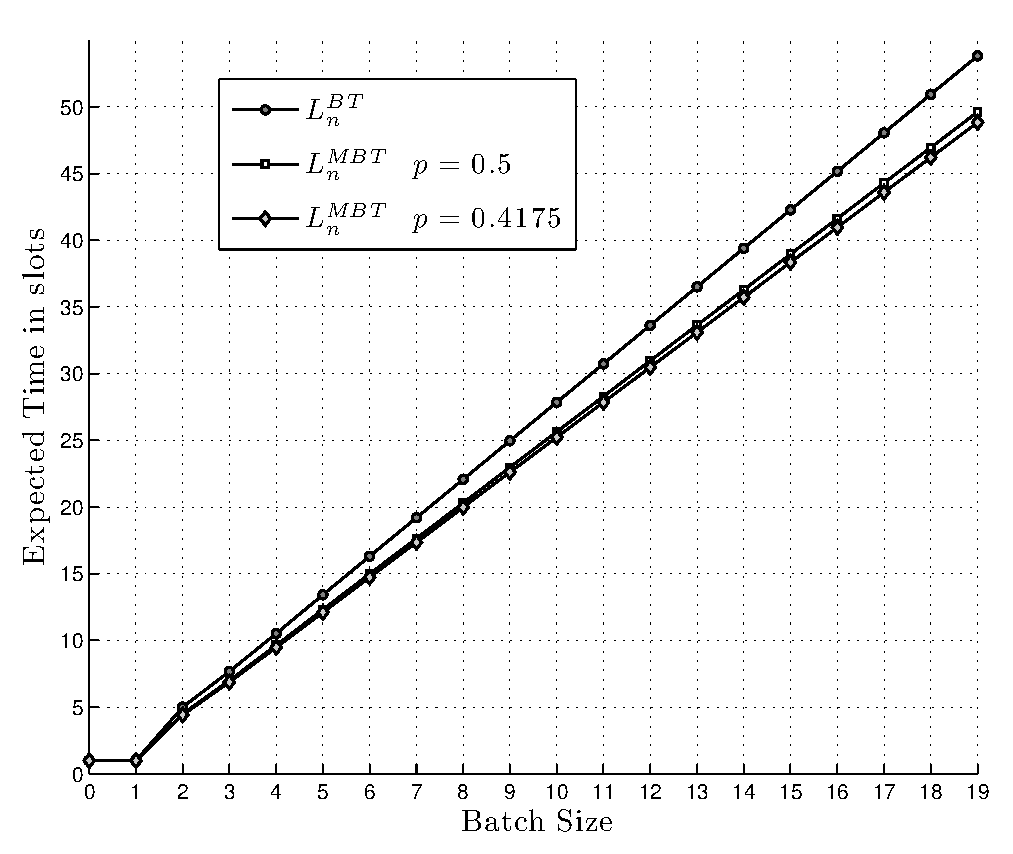
\includegraphics[scale=.7]{matlab/BTs/bin-trees-expected-time}
\caption[Expected Running time for tree algorithms]{Event probability for fixed $p=1/1024$.  $q_{0}(p,n) \approx  q_{1}(p,n)$ for $n=1023$}
\end{center}
\end{figure}

\begin{center}
\begin{tabular}{cccccc}
$L_{2} = 5.0000 $&$L_{7} = 19.2009 $  &$L_{12} = 32.6238 $  &$L_{17} = 48.0522 $  &$L_{22} = 62.4783 $ \\ 
$L_{3} = 7.6667 $&$L_{8} = 22.0854 $  &$L_{13} = 36.5096 $  &$L_{18} = 50.9375 $  &$L_{23} = 65.3636 $ \\ 
$L_{4} = 10.5238 $&$L_{9} = 24.9690 $  &$L_{14} = 39.3955 $  &$L_{19} = 53.8227 $  &$L_{24} = 68.2489 $ \\ 
$L_{5} = 13.4190 $&$L_{10} = 27.8532 $  &$L_{15} = 42.2812 $  &$L_{20} = 56.7078 $  &$L_{25} = 71.1344 $ \\  
$L_{6} = 16.3131 $&$L_{11} = 30.7382 $  &$L_{16} = 45.1668 $  &$L_{21} = 59.5930 $  &$L_{26} = 74.0198 $ \\  
\end{tabular} 
\end{center}


Considering the efficiency $\eta_{n}=n/L_{n}$ (messages over slots) we have a decreasing serie $\eta_{1}=1$, $\eta_{2}=0.40$, $\eta_{3}=0.3913$, \dots, $\eta_{16}=0.3542$ , \dots, $\eta_{31}=0.3505$. It can be shown \cite{capetanakis} that $\eta_{\infty} \approx 0.347$.\\

Since the algorithm is much more efficient in solving small batches respect to large ones we would prefer to have (ideally)  $n$ batches of size 1 rather than 1 batch of size $n$.\\
So knowing exactly the cardinality $n$ of the initial batch $\mathcal{B}$ can be used to split the nodes into small groups and resolve them faster. \\This is the idea behind many improvements over the basic binary tree algorithm and it shows the importance of having an accurate estimate of $n$ when the cardinality is initially unknown.

\begin{figure}
\centering
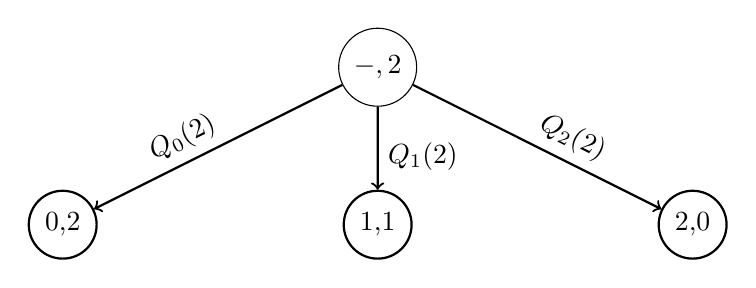
\begin{tikzpicture}[level/.style={->,thick,level distance = 20mm, sibling distance=40mm/#1}]

\node [circle,draw] (z) {$-,2$}
  {child{node [circle,draw] (a) {0,2} edge from parent
            node[ sloped, above, pos=.6] {$Q_{0}(2)$}}
  child {node [circle,draw] (b) {1,1} edge from parent
            node[ right, pos=.6] {$Q_{1}(2)$}}
  child {node [circle,draw] (c) {2,0}{child [grow=up]{node {} edge from parent [draw=none]}} edge from parent
            node[ sloped, above, pos=.6] {$Q_{2}(2)$}}
};
\end{tikzpicture}
\caption[\emph{BT}: Batch split probabilities]{Transaction probabilities to split a set of 2 elements into two sets with $i$, $j$ elements}
\end{figure}

\subsubsection{Example}

\begin{figure}[htbp!]
\centering
\ovalbox{
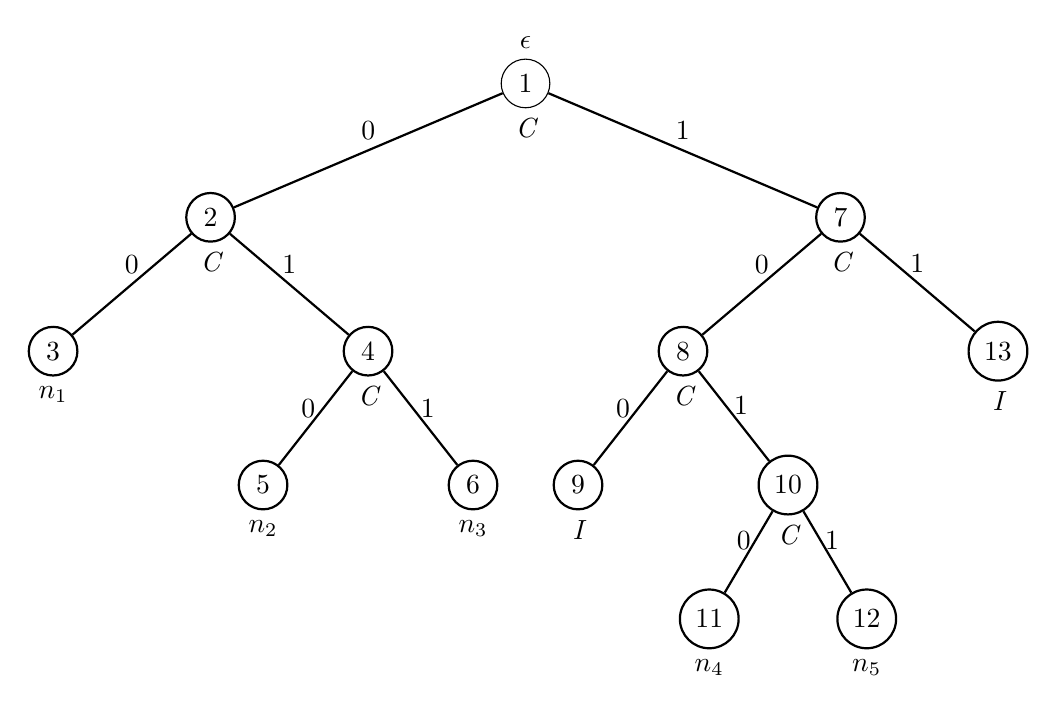
\begin{tikzpicture}[level/.style={thick,level distance = 17mm, sibling distance=80mm/#1}]

\node [circle,draw,label=below:\itshape C,label=above:$\epsilon$] (r){1}{
  	child{node [circle,draw,label=below:\itshape C] {2} {
		child{ node [circle,draw,label=below:$n_{1}$] {3} edge from parent node[ above, pos=.5] {0}
			}
		child{ node [circle,draw, label=below:\itshape C] {4}{		
			child{ node [circle,draw,label=below:$n_{2}$] {5} edge from parent node[ above, pos=.6] {0}}
			child{ node [circle,draw,label=below:$n_{3}$] {6} edge from parent node[ above, pos=.6] {1}}
			} edge from parent node[ above, pos=.5] {1}}
			} edge from parent node[above, pos=.5] {0}
  		}
  	child {node [circle,draw, label=below:\itshape C] {7}{
		child{ node [circle,draw, label=below:\itshape C] {8}{
			child{ node [circle,draw,label=below:\itshape I ] {9} edge from parent node[ above, pos=.6] {0}}
			child{ node [circle,draw,label=below:\itshape C] (s10){10} {
				child{ node [circle,draw,label=below:$n_{4}$] {11} edge from parent node[ above, pos=.6] {0}}
				child{ node [circle,draw,label=below:$n_{5}$] (s12){12} edge from parent node[above, pos=.6]{1} }
			}edge from parent node[ above, pos=.6] {1}}
		} edge from parent node[ above, pos=.5] {0}}
		child{ node [circle,draw,label=below:\itshape I ] {13} edge from parent node[ above, pos=.5] {1}}
		} edge from parentnode[ above, pos=.5] {1}
	}
	
};
\end{tikzpicture}
}
\caption[\emph{BT}: Basic binary tree example]{An istance of the binary tree algorithm for $n=5$ nodes. The number inside the each circle identifies the slot number. The label below identifies the event occurring: \textit{I} for \emph{idle}, \textit{C} for \emph{collision}, $n_{i}$ for resolution of node $i$. 0/1 branches is analogous to head/tail.}.
\label{example-bbt}
\end{figure}

In Figure \ref{example-bbt} we provide an example to further investigate the behavior of the algorithm. We notice that the instance start with a collision in slot 1. Then nodes $n_{1}$, $n_{2}$, $n_{3}$ decide to proceed with a retransmission while $n_{4}$, $n_{5}$ remain idle. In slot 2 we see another collision, after it $n_{1}$ decide to transmit again while $n_{2}$ and $ n_{3}$ to stay quiet. In slot 3 we have the first resolution, $n_{1}$ send successfully its message and won't no more take part to the collision resolution.\\
We notice that we can know the cardinality of a collision only after it has been fully  resolved. For example we know only after slot 6 that the collision in slot 2 involved 3 nodes.\\

\subsubsection{Nodes addresses}

Looking carefully to the tree you can see that each node resolved is characterized by an \emph{address}: the path from the root to node $n_{i}$ gives  a string of bits. For example node $n_{4}$'s address has as prefix 1010. The prefix in this case can be equivalent to the address but, in a more general case, node address can be a longer string. Assuming in fact that node $n_{4}$'s full address is the 8 bit long string 10100010, running the algorithm brings to the discovery of only the first 4 bits since the collision become resolved without requiring further split of the batch and deeper collision tree investigation (collision in level $t$ provokes a split and a deeper investigation in the tree at level $t+1$ and it requires to consider bit $t+1$ of the nodes' addresses).\\

\subsubsection{Tree traversal rules}

\textcolor{red}{
The inquirer must provide feedback about the event in a slot but tree walking can be either explicit or implicit. It is explicit if, with feedback, the reader provide also the address in the root of the currently enabled sub-tree. Otherwise it is said to be implicit and each node compute autonomously the new enabled sub-tree.}\\
We assume, following the conventional approach, to visit the tree in pre-order, giving precedence to sub-trees starting with 0.\\
Initially all nodes are enabled so the prefix is the empty string $\epsilon=b_{1..0}$, the root address. $\epsilon$ is considered to be prefix of any string.\\
Let $b_{1..k}$, with $b_{i} \in \{0,1\}$, $k \geq0$, be the current enabled $k$-bit prefix and \emph{event} $\in \{I,S,C\}$.\\
The possible cases are: \textcolor{red}{qui incasino un po' le cose con una notazione un po' imprecisa}
\begin{enumerate}[i.]
\item \emph{event} is $C$: no matter about $b_{1..k}$, next enabled interval will be $b_{1..k}0$;
\item \emph{event} is not $C$ and $b_{k}=0$: we successfully resolved the left part of the sub-tree, now we will look for right one. Next enabled prefix will be $b_{1..k-1}1$;
\item \emph{event} is not $C$ and $b_{k}=1$: we completed the  resolution of a left sub-tree, now we will look in the way back to the root for the first right sub-tree still unresolved. Let $t$ be $ \arg\underset{i \in 1..k}{\max}|b_{i}=0$ (or $t\gets 0$ if $b_{1..k}$ having 1 or more 1), in other words the position of the right most 0 in the prefix, if any. The new enabled interval will be $b_{t-1}1$. You can see this rule applied after slot 6 and 12 in the example;
\item termination condition is checking $b_{1..k}=\epsilon$.
\end{enumerate}

\subsubsection{\textcolor{red}{Real value approach}}
\label{realvalueapproach}
\textcolor{red}{Decidere se inserire o meno le considerazioni sulla visione degli indirizzi (alias ID) dei nodi come numeri reali tra 0 e 1 e della risoluzione come intervalli reali abilitati contenenti un solo nodo. Utile per collegarsi a popovski/cidon e alla suddivisione in insiemi in generale}\\
Every length binary string can be also interpreted as a real number in the interval $[0,1)$
\begin{equation*}
11001 \leftrightarrow 1 \cdot 2^{-1} + 1 \cdot 2^{-2} + 0 \cdot 2^{-3} + 0 \cdot 2^{-4} +1 \cdot 2^{-5} 
\end{equation*}
by associating to each position in the string a different power of 2.\\
In general a given a string $\mathbf{b_{i}}=(b_{i1}b_{i2}b_{i3}\ldots)$, with $b_{ij} \in \{0,1\}$, can be associated to a real number $r_{i} \in [0,1)$ by a bijective map $r$:\\

\begin{equation}
r_{i}=r(\mathbf{b_{i}})=\sum_{j=1}^{\infty} \ \frac{b_{ij}}{2^{j}}
\end{equation}

So we could think, instead of tossing a coin only when needed, to initially flip a coin, in the same manner, $L$ times to get a $L$-bits randomized string.
In this way each node can be immediately be assigned to a set of length $2^{-L}$. There are $2^{L}$ relatively ordered distinct sets in the interval [0,1).\\
Given a finite control string $\mathbf{a_{i}}=(a_{i1}a_{i2}\ldots a_{ik})$, it enables all the nodes identified by real number $x$ within the interval:
\begin{equation}
	r(\mathbf{a_{i}})\leq x <r(\mathbf{a_{i}})+2^{-k}
\end{equation}

\textcolor{red}{QUESTA OSSERVAZIONE é SOLO FRUTTO DEL MIO SACCO E MI SEMBRAVA INTERESSANTE.\\
An interesting observation is that the distribution of the nodes into the real interval depends upon $p$, the probability  to obtain 0 or 1 tossing a biased coin.
è interessante perchè per il basic binary tree p ottimo è 0.5 per cui si ottiene una distribuzione sperabilmente uniforme dei nodi (o poisson?). Mentre 0.5 non è ottimo per il Modified binary tree: p ottimo 0.4175. quindi la distribuzione migliore per il MBT è una specie di esponenziale discreta e la profondità dell'albero aumenta più ci si avvicina a 1. Questo è quello che mi dice l'intuizione e non ho visto scritto da nessuna parte (magari sul paper orginale del MBT c'è). per cui il MBT non può essere utilizzato banalmente per fare stime tramite una risoluzione parziale di un qualunque sotto intervallo $[0,x)$ con k nodi poichè $n \neq \frac{k}{x} $ (popovski) a meno che non sia nota la distribuzione dei nodi $f(x) $e si normalizzi per $f(x)$ al posto che $x$. 
NOTA: in popovski pg 295  dicono \emph{To summarize, we can say that without any modification, the BT (or the MBT) algorithm offers a way to estimate the unknown conflict multiplicity}. il che è ok ma solo se MBT usa p=0.5
per cui $f(x)=x$. studiare $f(x,p)$?}
\subsection{Modified Binary Tree}

Modified binary tree is a simple way to improve the basic variant for the binary tree algorithm.\\ The observation is that, during the tree traversal, sometimes we know in advance if the next slot there will be collided. This happens when, after a collided slot ($\tau$), we get and idle slot ($\tau+1$) in the left branch of the binary tree: visiting the right branch ($\tau+2$) we will get a collision for sure.\\
In fact in slot ($\tau$) we know that in the sub-tree there are at least 2 nodes and none of them owns to the left-branch sub-tree ($\tau+1$). So they must be in the right sub-tree and when enabled to transmit ($\tau+2$) transmissions will disrupt.
Solution is to keep previous node ($\tau+2$) as a virtual node, to skip it, and continue visiting node ($\tau+1$).$sibling$.$leftchild$ in slot $(\tau+2)$.
This let us save a slot.\\

\begin{figure}[htbp!]
\centering
\ovalbox{
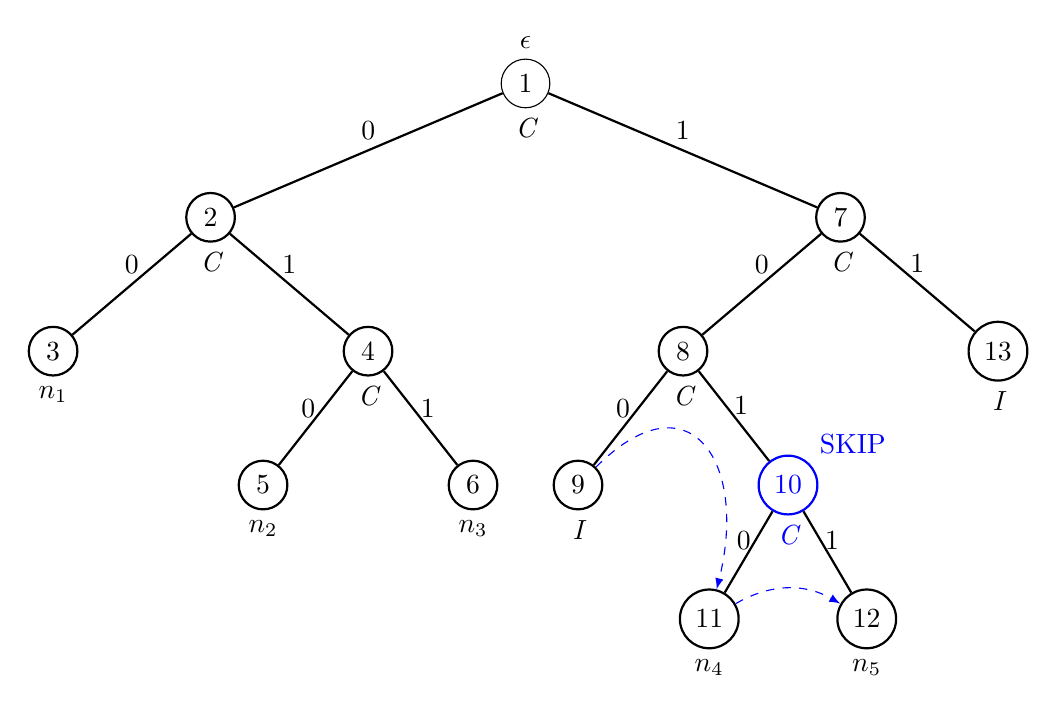
\begin{tikzpicture}[scale=1, level/.style={thick,level distance = 17mm, sibling distance=80mm/#1}]

\node [circle,draw,label=below:\itshape C,label=above:$\epsilon$] (r){1}{
  	child{node [circle,draw,label=below:\itshape C] {2} {
		child{ node [circle,draw,label=below:$n_{1}$] {3} edge from parent node[ above, pos=.5] {0}
			}
		child{ node [circle,draw, label=below:\itshape C] {4}{		
			child{ node [circle,draw,label=below:$n_{2}$] {5} edge from parent node[ above, pos=.6] {0}}
			child{ node [circle,draw,label=below:$n_{3}$] {6} edge from parent node[ above, pos=.6] {1}}
			} edge from parent node[ above, pos=.5] {1}}
			} edge from parent node[above, pos=.5] {0}
  		}
  	child {node [circle,draw, label=below:\itshape C] {7}{
		child{ node [circle,draw, label=below:\itshape C] (s8) {8}{
			child{ node [circle,draw,label=below:\itshape I ] (s9){9} edge from parent node[ above, pos=.6] (s89){0}}
			child{ node [circle,draw,blue,label=below:\itshape \textcolor{blue}{C},label=45:\textcolor{blue}{SKIP}] (s10){10} {
				child{ node [circle,draw,label=below:$n_{4}$] (s11){11} edge from parent node[ above, pos=.6] (s1011){0}}
				child{ node [circle,draw,label=below:$n_{5}$] (s12){12} edge from parent node[above, pos=.6]{1} }
			}edge from parent node[ above, pos=.6] {1}}
		} edge from parent node[ above, pos=.5] {0}}
		child{ node [circle,draw,label=below:\itshape I ] {13} edge from parent node[ above, pos=.5] {1}}
		} edge from parent node[ above, pos=.5] {1}
	}	
};
%scale=0.8
%\draw [-latex,blue,thin,dashed] (s9) .. controls ++(46:1.6) and ++(0.5,1.6) .. (s11);
%\draw [-latex,blue,thin,dashed] (s11) to [bend left ](s12);
%scale =1;
\draw [-latex,blue,thin,dashed] (s9) .. controls ++(45:2) and ++(0.5,2) .. (s11);
\draw [-latex,blue,thin,dashed] (s11) to [bend left ](s12);
\end{tikzpicture}
}
\caption[\emph{MBT}: Modified binary tree example]{Same example as in Figure \ref{example-bbt} but using \algname{MBT}: tree structure do not change but node 10 is skipped in the traversal. $\tau=8$}
\label{example-mbt}
\end{figure}

Expected time analysis is analogous  to section \ref{basicbinarytreedescription}. \textcolor{red}{The only difference is that after a collision, if we get and idle slot, we will skip the ``next one'' (and we won't pay for it). So we can see that the expected slot cost is $\left[1 \cdot \bigl(1-Q_{0}(n)\bigr)+ 0\cdot Q_{0}(n)\right]$}. Then\\
\begin{equation}
L_{n}^{MBT} = \bigl(1 - Q_{0}(n)\bigr)+\sum_{i=0}^{n} Q_{i}(n) (L_{i}^{MBT}+L_{n-i}^{MBT})
\end{equation}
with
\begin{equation*}
L_{0}^{MBT} = L_{1}^{MBT}  = 1
\end{equation*}
Intuitively in this case, since an higher probability to stay silent, reduces the expected slot cost, optimal transmit probability won't no more be $1/2$. At the same time lowering the transmit probability will increase the number of (wasted) idle slots. So the new optimal probability $p$ will be somewhere in the interval (0,1/2).\\
It can be shown\footnote{  J.L Massey,\emph{Collision-Resolution Algorithms and Random-Access Communications}, CISM Courses and Lectures, vol. 265, pp. 73–137. Springer, Berlin (1981)} that best achievable result is for $p=0.4175$ and, with this $p$, efficiency $\eta \approx 0.381$ as $n \to \infty$ which is asintotically +10\% faster than basic BT.\\
In general we have: 
\begin{equation}
L_{n}\leq C \cdot n +1 \qquad \textrm{where} \qquad C=2.622
\end{equation}
Not using optimal probability for $p$ but 1/2 results, for large $n$, in about 0.2\% peak performance loss  ($C=2.667$) which is a really moderate decrease.\\
What is even more important  is that 0.4175 is close to the optimal bias for small $n$ as well.
\chapter{Batch Size Estimate Techniques}
\label{ch:Batch Size Estimate Techniques}
We present here some noteworthy techniques for batch size estimate that can be found in literature.
If the technique was not already identified by a name or associated to a acronym we used the name of one authors as reference.\\

In general, we assume not to have any \emph{a priori} statistical knowledge about the multiplicity of the nodes involved in a collision. So estimation techniques must provide efficient ways to obtain an estimate for the general zero-knowledge scenario.\\
\section{CBT}
\label{cbt-estimation}
The most simple idea to obtain an estimate of the batch size could be to solve a minimum amount of nodes to obtain an estimate. This can be done, for example, by using deterministic algorithms such as CBT.\\
CBT is a partial resolution algorithm since only a fraction of the packets of the batch are successfully transmitted.
The clipped binary tree algorithm is identical to the modified binary tree algorithm (with $p=1/2$ since we require the nodes to be uniformly distributed in the interval [0,1) ) except that it is stopped (the tree is clipped) whenever two consecutive successful transmissions follow a conflict.\\
When the algorithm stops we know than the last two nodes resolved owns to the same level $i$ of the tree (root is at level=0).\\
We could think to obtain an estimate as:
\begin{equation}
\hat{n}\gets2^{i}
\end{equation}
\begin{comment}
The idea is interesting but the fact of considering recursively subsets of subsets of the initial batch brings to disastrous performance: as reported in \cite{greenberg87}, second and all higher moments of this estimate are infinite.\\
So this simple method is not good to obtain an estimate. 
\end{comment}

\begin{figure}[H]
\centering
\ovalbox{
\begin{tikzpicture}[level/.style={thick,level distance = 17mm, sibling distance=80mm/#1}]

\node [circle,draw,label=below:\itshape C,label=above:$\epsilon$] (r){1}{
  	child{node [circle,draw,label=below:\itshape C] {2} {
		child{ node [circle,draw,label=below:$n_{1}$] {3} edge from parent node[ above, pos=.5] {0}
			}
		child{ node [circle,draw, label=below:\itshape C] {4}{		
			child{ node [circle,draw,label=below:$n_{2}$] {5} edge from parent node[ above, pos=.6] {0}}
			child{ node [circle,draw,label=below:$n_{3}$] {6} edge from parent node[ above, pos=.6] {1}}
			} edge from parent node[ above, pos=.5] {1}}
			} edge from parent node[above, pos=.5] {0}
  		}
	child {node {} {child {node {} edge from parent[draw=none]} child {node {} edge from parent[draw=none]}}edge from parent[draw=none]}
};
\end{tikzpicture}
}
\caption[\emph{CBT}: example]{ Same example as in Figure \ref{example-bbt} but resolution using CBT ends up after two consecutive successful transmissions.}
\end{figure}

Experimental results show that the variance of the obtained estimate is extremely high and the resulting accuracy is really poor.\\ 
This is due to the fact that the batch of interest we use for the estimate becomes, at each level, smaller and smaller: the estimate, even for huge sizes, depends only on very few (3-5) nodes (those with lower addresses). So estimate is quite unstable.\\
Results are reported in Appendix in tables  \ref{CBT-table-1}. Notice how slowly the distribution probability decrease.
\section{Cidon}

Cidon and Sidi proposed this approach in \cite{cidon}. In this work they describe a complete resolution algorithm based on two phases:
 
\begin{enumerate}
\item to get an estimate of the initial batch using a partial deterministic resolution scheme. 
\item to perform an optimized complete deterministic resolution basing on the results of phase 1. 
\end{enumerate}

The strategy adopted to obtain the estimate is to resolve a small portion of the batch and to accumulate the number of successful transmission resulted.\\

Initially we fix a probability $\pc$ that determines how the whole batch is split at the very first time.\\
We named it $\pc$ to underlined than this initial choice reflects on the expected accuracy of the resulting estimate.\\

As usual we have initially a batch $\mathcal{B}$ of unknown size $n$.
At the beginning of the algorithm each node chooses to transmit with probability $\pc$. Thus the $n$ nodes are partitioned into two set $\mathcal{E}$ and $\mathcal{D}$, where $\mathcal{E}$ consist of those that transmitted and $\mathcal{D}$ the rest. Clearly, $|\mathcal{E}|+|\mathcal{D}|=n$. If the resulting slot is empty or contains a successful transmission, we conclude that $|\mathcal{E}|=0$  or $|\mathcal{E}|=1$, respectively. If a conflict occurs, it is known that $|\mathcal{E}|\geq2$, and the nodes in $\mathcal{E}$ use a complete batch resolution algorithm to resolve the conflicts among the nodes in $\mathcal{E}$. At the end of this part we know the exact value of $\mathcal{E}$ by accumulating the number of successful transmissions during the resolution. We call this counter $j$.
So, after this estimation phase, since we expect that the nodes are uniformly distributed in the real interval [0,1) and we solved the first part of the interval from 0 to $\pc$ we found that our expected density can be supposed to be $\frac{j}{\pc}$.
Then we simply compute our estimate $\hat{n}$ as: 

\begin{equation}
\hat{n} \gets \frac{j}{\pc}
\end{equation}
In this  case, since we already resolved the nodes in $\mathcal{E}$, we are more interested only in the cardinality of the remaining batch to solve $\mathcal{D}$ which we can compute as:

\begin{equation}
\hat{k}=E[size(\mathcal{D})] \gets  \frac{j}{\pc}(1-\pc)
\end{equation}
 

\begin{algorithm}[h!]
\begin{algorithmic}[1]
	\REQUIRE $\pc$, fraction of the whole batch to solve
	\STATE \COMMENT{Phase 1}
	\STATE each node flip a coin getting 0 with probability $\pc$, 1 otherwise
	\STATE $\mathcal{E} \gets$ \{ nodes that flipped 0\}
	\STATE $\mathcal{D} \gets$ \{ nodes that flipped 1\}
	\STATE \algname{Complete collision resolution ($\mathcal{E}$) }
	\STATE  $\hat{k} \gets |\mathcal{E}|/\pc$
	\STATE \COMMENT{Phase 2}
	\STATE \algname{Optimized complete collision resolution ($\mathcal{D}$,$\hat{k}$, $\pc$) }
	\end{algorithmic}
\caption{\algname{Cidon}}
\label{alg-cidon}
\end{algorithm}

Note that $|\mathcal{E}| = 0$ does not imply $|\mathcal{D}| = 0$ so a complete resolution algorithm has always to be performed on $\mathcal{D}$.
Recalling subsection ``Real Value Approach'' in \ref{realvalueapproach}, operation on line 2 in Alg. \ref{alg-cidon} is equivalent to force each node to generate a unique ID expressed as a fixed length real value in the interval [0,1).\\
Following Figure \ref{cidon-nodes-id} show the case providing a simple example.
\begin{figure}[H]
    \centering
    \ovalbox{
    \begin{tikzpicture}
    \draw [thick, [-)] (0,0) node[label=below:0] {}-- (10,0) node[label=below:1] {};
    
    \foreach \x / \y in{1/$n_{1}$,2/$n_{2}$,3.5/$n_{3}$,4/$n_{4}$,5.5/$n_{5}$,7.6/$n_{6}$,9.2/$n_{7}$}
    \draw[->] (\x,1) node [label=above:\y]{} -- (\x,0.3);
    
    % 
    \draw[->] (3,-1) node [label=below:$<\pc\leq$]{} -- (3,-0.3);
    \draw[snake=crosses, very thick] (3,0) node [label=above:0.3] {}-- (3.2,0);
    
    \end{tikzpicture}
    }
    \caption[\emph{Cidon}: initial split]{In this example $\pc=0.3$. At the beginning of the algorithm each node generate its own ID. Nodes whose ID is less than $\pc$ owns to $\mathcal{E}$. Nodes whose ID is greater or equal to $\pc$ owns to $\mathcal{D}$. Estimate of the batch returns $\lceil 2/0.3\rceil=7$ which, in this case, is the exact size of the batch.}
    \label{cidon-nodes-id}
\end{figure}
 
 Procedure \algname{Complete collision resolution ($\mathcal{E}$) } identifies any procedure able to resolve all the nodes in $\mathcal{E}$ allowing them to successfully transmit their messages while \algname{Optimized complete collision resolution ($\mathcal{D}$,$\hat{k}$, $\pc$) } identifies an optimized way to resolve the batch $\mathcal{D}$: speedup is allowed by the knowledge of its expected multiplicity.\\
 
 Expected running time depends on the BRA used but in general can be considered $O(\pc n)$: time is linear in the size of $\mathcal{E}$.

\subsection{Estimate accuracy}
\label{cidon-estimate-accuracy}

In the original paper \cite{cidon} there is no detailed analysis of the behavior of the algorithm but it is only shown the following fact: as $n$ grows the estimator becomes more accurate.\\
    
Let $J$ be an integer random variable which expresses the number of nodes in $\mathcal{E}$. Given a batch of size $n$, $J$ is binomially distributed with parameter $\pc$. It can be thought as the probability distribution to put $j$ among  $n$ nodes in two bins choosing with probability $\pc$ the first one and $1-\pc$ the other one.  Therefore, we have the following:

\begin{enumerate}[1)]
\item \begin{equation}P(J=j|n)={n \choose j}\pc^{j}(1-\pc)^{n-j}
           \label{cidon-J}\end{equation}
\item \begin{equation}E[J|n]=n\pc\label{cidon-e-estimate}\end{equation}
\item \begin{equation}\textrm{var}(J|n)=n\pc(1-\pc)\end{equation}
\end{enumerate}

By applying Chebychev's Inequality \eqref{eq:cheby},  we have for any $\epsilon>0$
 
 \begin{equation}
P\Bigl( \left| J-n\pc\right| \geq \epsilon n \,|\, n \Bigr) \leq \frac{\pc(1-\pc)}{\epsilon^{2}n}
\label{eq:cidon-cheby}
 \end{equation}
 Let $\hat{N}$ be a real-valued random variable that expresses our estimate upon $n$. Then from \eqref{cidon-J} - \eqref{eq:cidon-cheby}:

\begin{enumerate}[1)]
\item \begin{equation}P\left(\hat{N}=n|n\right)={n \choose j}\pc^{j}(1-\pc)^{n-j} \quad \textrm{with} \quad \hat{n}=j/\pc, \quad 0\leq j\leq n\end{equation}
\item \begin{equation}E[\hat{N}|n]=n\end{equation}
\item  \begin{equation}
P\left( \left| \frac{\hat{N}}{n}-1\right| \geq \epsilon  \,\big|\, n \right) \leq \frac{1-\pc}{\epsilon^{2}n\pc}
 \end{equation}
\end{enumerate}
\clearpage
\section{Greenberg}

Let, as usual, $n$ be our batch size.\\
Basic Greenberg algorithm's strategy is to search for \emph{a power of 2} that is close to $n$ with high probability.\\
The probabilistic test is defined to look for $\hat{n}$ which tries to satisfy:\\
\begin{equation}
\hat{n}\geq 2^{i} \approx n
\end{equation}
Let each of the $n$ conflicting stations either transmit or not transmit in accordance with whether the outcome of a biased binary coin is 0 or 1. The coin is biased to turn up 0 with probability  $2^{-i}$ and 1 with complementary probability. Since the expected number of transmitters is $2^{-i}n$, having a conflict as event supports the hypothesis that $n\geq2^{i}$.\\
Using this test repeatedly with $i=1, 2, 3, \ldots$ leads to the Greenberg \emph{base 2 estimation algorithm}.\\
Each of the conflicting stations executes Algorithm (\ref{alg-greenberg}), resulting in a string of collisions whose lenght determines $\hat{n}$.\\

As $i$ increases, the probability that at most one node transmits increases monotonically and approaces 1 extremely rapidly as $i$ increases past $\log_{2}n$ so we expect $i$ is close to $\log_{2}n$.\\

\begin{algorithm}[H]
\begin{algorithmic}
\STATE $i\gets 0$
\REPEAT
	\STATE $i\gets i+1$
	\STATE choose to transmit with probability $2^{-i}$
\UNTIL {no collision occurs}
\STATE $\hat{n} \gets 2^{i}$
\end{algorithmic}
\caption{\algname{Basic Greenberg}}
\label{alg-greenberg}
\end{algorithm}

The idea behind algorithm \ref{alg-greenberg} appears to be quite simple: as the algorithm goes on the initial unknown batch (of size $n$) comes progressively sliced into smaller pieces. Only the nodes virtually inside the slice are allowed to transmit. Slices get thinner and thinner until at most one node is contained in a slice. Figure \ref{fig:greeberg-split} intuitively tries to explain the idea.\\ 

\begin{figure}[htb!]
    \centering
    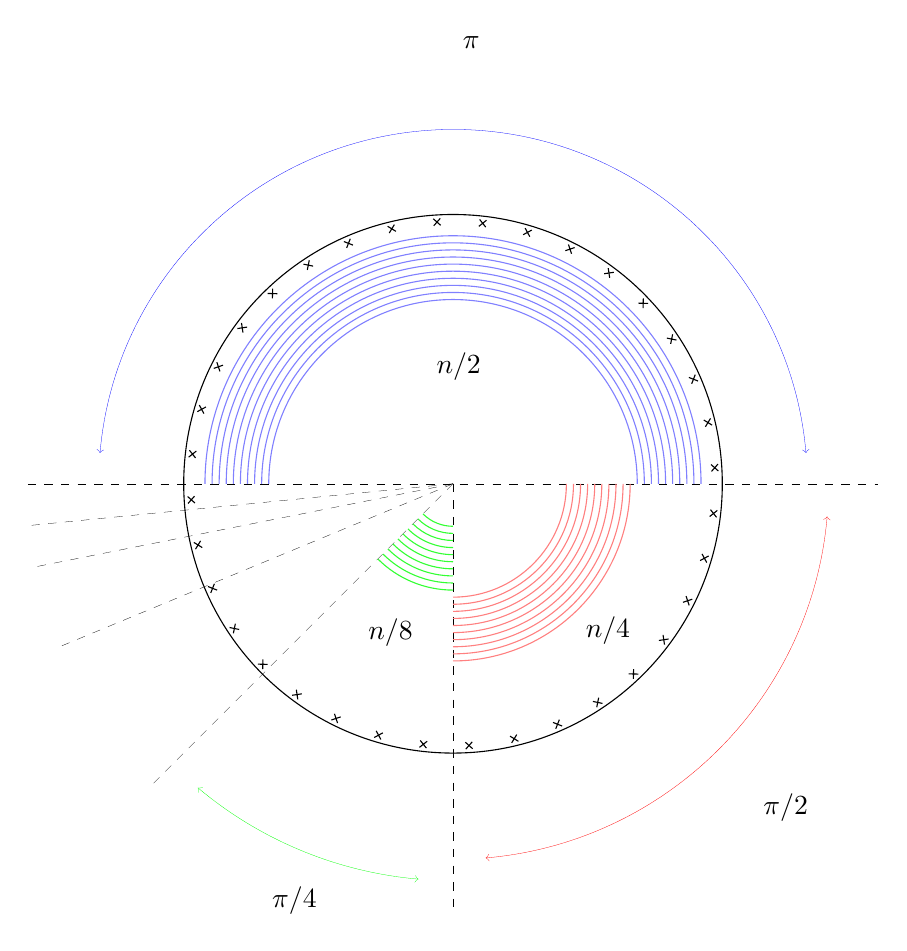
\begin{tikzpicture}[scale=0.9]  
        \draw (0, 0) circle (3.8cm);
        \foreach \x in {3.5,13.5,...,360}
        \draw[snake=crosses] (\x:3.7) --(\x:3.8);
       \draw[-,ultra thin,dashed] (180:6) to[] (0:6); 
       \draw[-,ultra thin,dashed] (0,0) to[] (-90:6);
       \draw[-,ultra thin,dashed] (0,0) to[] (-135:6);
       \draw[-,ultra thin,dashed] (0,0) to[] (-157.5:6);
       \draw[-,ultra thin,dashed] (0,0) to[] (-168.75:6); 
       \draw[-,ultra thin,dashed] (0,0) to[] (-174.375:6);  
        %arco rosso
        \foreach \x/\text in {1.6,1.7,...,2.5}
        \draw [-,thin,red!50] (0:\x) arc(0:-90:\x);
        %arco  blue
        \foreach \x/\text in {2.6,2.7,...,3.5}
        \draw [-,thin,blue!50] (0:\x) arc(0:180:\x); 
        %arco verde
        \foreach \x/\text in {.6,.7,...,1.5}
        \draw [-,thin,green!80] (-90:\x) arc(-90:-135:\x);

        \draw [<->,ultra thin,blue] (5:5) arc(5:175:5);
        \draw [<->,ultra thin,red] (-5:5.3) arc(-5:-85:5.3);
        \draw [<->,ultra thin,green] (-95:5.6) arc(-95:-130:5.6);
        
        \path[text width=3pt]
        (90:6)      node[above right] {$\pi$}  (95:2)      node[below] {$n/2$}
        (-45:6)      node[below right] {$\pi/2$} (-50:2.7)      node[right] {$n/4$}
        (-112.5:6)      node[below left] {$\pi/4$} (-118:2)      node[below left] {$n/8$};
    \end{tikzpicture}
    \caption[\emph{Basic Greenberg}: batch split idea]{Visually nodes can be thought to be uniformly distributed on the circumference of a circle. By performing Greenberg's algorithm we go and analyze each time a smaller sector (in this case the half of the previous one) of the circle and find when a sector contains only 1 or no nodes.  Not overlapping sectors are drawn to maintain the image simple but in general nodes gets redistributed to each step of the algorithm}
    \label{fig:greeberg-split}
\end{figure}

Expected running time is $O(log_{2}n)$. In particular, since in the SLOTTED ALOHA model considered in the paper reader feedback is supposed to be transmitted at the end of each transmission slot, expected running time can be expressed, in slot numbers, as $\approx 1+\log_{2}n$.\\

An important note is that the algorithm always involve all the nodes in the batch: in each stage of the algorithm each node has to take a choice if transmit or not. 
Each choice is independent of what the node did in the previous steps. \\ 
This is of great importance and allows $\hat{n}$ to have bounded moments: it can be shown for large $n$ that:
\begin{equation}
E[\hat{n}] \approx n\phi
\end{equation}
\begin{equation}
E[\hat{n}^{2}] \approx n\Phi
\end{equation}
where
\begin{equation}
\phi= \frac{1}{\log2} \int_{0}^{\infty} \! e^{-x}(1+x) \prod_{k=1}^{\infty}\bigl(1-e^{-2^{k}x}(1+2^{k}x)\bigr)x^{-2} \, dx = 0.91422\dots
\end{equation}

\begin{equation}
\Phi= \frac{1}{\log2} \int_{0}^{\infty} \! e^{-x}(1+x) \prod_{k=1}^{\infty}\bigl(1-e^{-2^{k}x}(1+2^{k}x)\bigr)x^{-3} \, dx =1.23278\dots
\end{equation}

\noindent $\phi$ and $\Phi$ where obtained in \cite{greenberg87} using advanced mathematical analysis supported by Mellin integral transform\footnote{in this work we only report these as final results, please refer to the original paper to see how $\phi$ and $\Phi$ where obtained.}.
In general $\phi$ and $\Phi$ depend on the size of the problem. We present Table \ref{table:phi-Phi} to provide an idea of the behavior of $\phi$ as function of $n$.\\

\begin{table}[H]
\caption[\emph{Basic Greenberg}: Expected Estimate]{Given a batch of size $n$ the expected estimate applying base 2 Greenberg is $E[\hat{n}|n]$. The ratio $E[\hat{n}|n]/n$ monotonically decreases and gets stable at $0.9142$. This shows that this estimate technique provide biased results.}
\begin{center}
\begin{tabular}{rD{.}{.}{5.2}D{.}{.}{1.4}}
 n & \multicolumn{1}{r}{$E[\hat{n}|n]$} & \multicolumn{1}{c}{$E[\hat{n}|n]/n$} \\ \hline \hline
1 &     2.00 &   2.0000 \\ 
2 &     2.56 &   1.2822 \\ 
4 &     4.21 &   1.0533 \\ 
8 &     7.89 &   0.9863 \\ 
16 &  15.20 &   0.9498 \\ 
32 &    29.82 &   0.9320 \\ 
64 &    59.08 &   0.9231 \\ 
128 &   117.59 &   0.9186 \\ 
256 &   234.60 &   0.9164 \\ 
512 &   468.64 &   0.9153 \\ 
1024 &   936.71 &   0.9148 \\ 
2048 &  1872.86 &   0.9145 \\ 
4096 &  3745.14 &   0.9143 \\ 
8192 &  7489.72 &   0.9143 \\ 
16384 & 14978.86 &   0.9142 \\ 
32768 & 29957.16 &   0.9142 \\ 
65536 & 59913.74 &   0.9142
\end{tabular}
\end{center}
\label{table:phi-Phi}
\end{table}
The fact that, for large $n$, $E[\hat{n}] \approx n\phi$ suggests treating $\hat{n}_{+} = \hat{n}/\phi$ as a estimate of n.\\


Interestingly, a simple variant of the estimation algorithm has disastrous performance. Consider the algorithm in which each station involved in the initial collision transmits to he channel with probability $\frac{1}{2}$. If this causes another collision, then those that just transmitted again transmit with probability $\frac{1}{2}$. The others drop out. This continues, with the stations continuing to try to transmit always being a subset of those that just transmitted, until there is no collision. Take $2^{i}$ as the estimate of the multiplicity of conflict where $i$ is the number of the steps until ther is no collision. It can be shown that the second and all higher moments of this estimate are infinite.

\subsection{base \emph{b} variant}

Using basic Algorithm \ref{alg-greenberg}, even though the expected value of $\hat{n}_{+}$ is quite close to $n$, $\hat{n}_{+}$ is likely to differ from $n$ by a factor of 2. In the original work a small generalization of the base 2 algorithm is proposed to remedy this limit: providing and estimate whose mean is  close to $n$ but whose  distribution peaks more sharply about the mean.\\
Simply it is suggested to use $b$ instead of 2 as base, with $1<b\leq2$.\\
\begin{algorithm}[H]
\begin{algorithmic}
\STATE $i\gets 0$
\REPEAT
	\STATE $i\gets i+1$
	\STATE transmit with probability $b^{-i}$
\UNTIL {no collision occurs}
\STATE $\hat{n}(b) \gets 2^{i}$
\STATE $\hat{n}_{+}(b) \gets \hat{n}(b)/\phi(b)$
\end{algorithmic}
\caption{\algname{base \emph{b} Greenberg}}
\label{alg-greenberg-base-b}
\end{algorithm}

$\phi(b)$ corrects the bias of the estimator. $\phi(b)$ is the optimal correction when $n$ is large.
Looking at Table \ref{table:greenberg-b-phi} you can notice how smaller $b$ results in smaller $\phi(b)$. This means that $b$ deeply biases the estimate: if $b^{'} < b^{''}$ then $E[\hat{n}(b^{'})] < E[\hat{n}(b^{''})]$.\\ This is a result of the following fact: let $i^{''}$ be the expected slot the base $b^{''}$ algorithm will end up given a batch size $n$, then $i^{''} \leq log_{b^{''}} n$. Let $i^{'}$ be the same for $b^{''}$. If $b^{'} < b^{''}$ then $b^{'i^{'}} > b^{''i^{''}}$ \symbolfootnote[2]{This comes from experimental observations.}

%nota della tabella, assicurarsi che sia nella stessa pagina

\begin{table}[H]
\caption[\emph{Greenberg}: different $b$ summary]{Following table shows how $\phi$ and ``Expected algorithm \ref{alg-greenberg-base-b} cost in slots'' vary for different $b$. Expected cost ($\lesssim \log_{b}n$) is expressed as a multiplicative factor for the basic Greenberg algorithm cost ($\lesssim \log_{2}n$).}
\label{table:greenberg-b-phi}
\begin{center}
\begin{threeparttable}
\begin{tabular}{lccl}
$b$ & $\phi(b)$\tnote{a} &\,\,\,& Expected cost in slots-1\\
\toprule
2          & $\approx 0.9142$ && $\lesssim 1 \qquad\,\,\, \times \log_{2} n$\\
1.1       & $\approx 0.3484$ && $ \lesssim 7.27$\\
1.01     & $\approx 0.1960$ && $ \lesssim 69.66$\\
1.001   & $\approx 0.1348$ && $ \lesssim 693.49$\\
1.0001 & $\approx 0.1027$ && $ \lesssim 6931.81$\\
\bottomrule
\end{tabular}
\begin{tablenotes}
\item [a] {\footnotesize \smaller Code used to compute $\phi(b)$ is provided in Appendix \ref{sec:greenberg-moments}}
\end{tablenotes}
\end{threeparttable}
\end{center}
\end{table}

It can be shown \cite{greenberg87} that, \emph{for all n greater than some constant $n_{0}(b)$}
\begin{enumerate}
\item \begin{equation} 
		\left |\frac{E[\hat{n}_{+}(b)]}{n}-1 \right | < \epsilon(b) 
	  \end{equation}
\item \begin{equation}
		\frac{\sigma\bigl(\hat{n}_{+}(b)\bigr)}{n}< \epsilon(b)
	\end{equation}
\end{enumerate}
\emph{where $\epsilon(b) \to 0$ as $b \to 1$.}

In other words when $b \to 1$ and $n$ is large the estimate becomes unbiased and variance goes to 0: we have ideally a perfect estimator.\\
Our experimental results showed that this estimator is not so good for real life scenarios.  




\section{Window Based}
\chapter{Performance Analysis}
\label{ch:Performance Analysis}
We investigated about a fast algorithms for multiplicity estimation.\\

\section{Cidon Evaluation}

\begin{equation*}
\end{equation*}
We remember from section \ref{cidon-estimate-accuracy} that
\begin{equation*}P(J=j|n)={n \choose j}\pc^{j}(1-\pc)^{n-j}\end{equation*}
and
\begin{equation*}\hat{n}=j/p\end{equation*}
Note that  in Alg. \ref{alg-cidon} (Cidon) we have $\pc$ \emph{a priori} fixed since it is an input parameter of the algorithm. So $J$ is a binomial distribution with parameters $B(n,\pc)$ and recalling \eqref{cidon-e-estimate}
we get:
\begin{equation}
E[\hat{n}|n,\pc]=\frac{1}{\pc}E\left[j|n,\pc\right]=n, \qquad \forall \,\pc
\end{equation}
This shows that Cidon provides an unbiased estimator ($E[\hat{n}|n]=n$) independently from $\pc$: $\pc$ influences only the variance of the estimator. 

\begin{equation}
\begin{split}
\textrm{var}(\hat{n}|n) & =E[\hat{n}^{2}|n]- E[\hat{n}|n]^{2}\\
& = \frac{1}{\pc^{2}}E[j^{2}|n] - n^{2}\\
& = \frac{n\pc(1-\pc)+n^{2}\pc^{2}}{\pc^{2}}- n^{2}\\
& =  \frac{n}{\pc}-n
\end{split}
\end{equation}

\begin{figure}[htbp]
\begin{center}
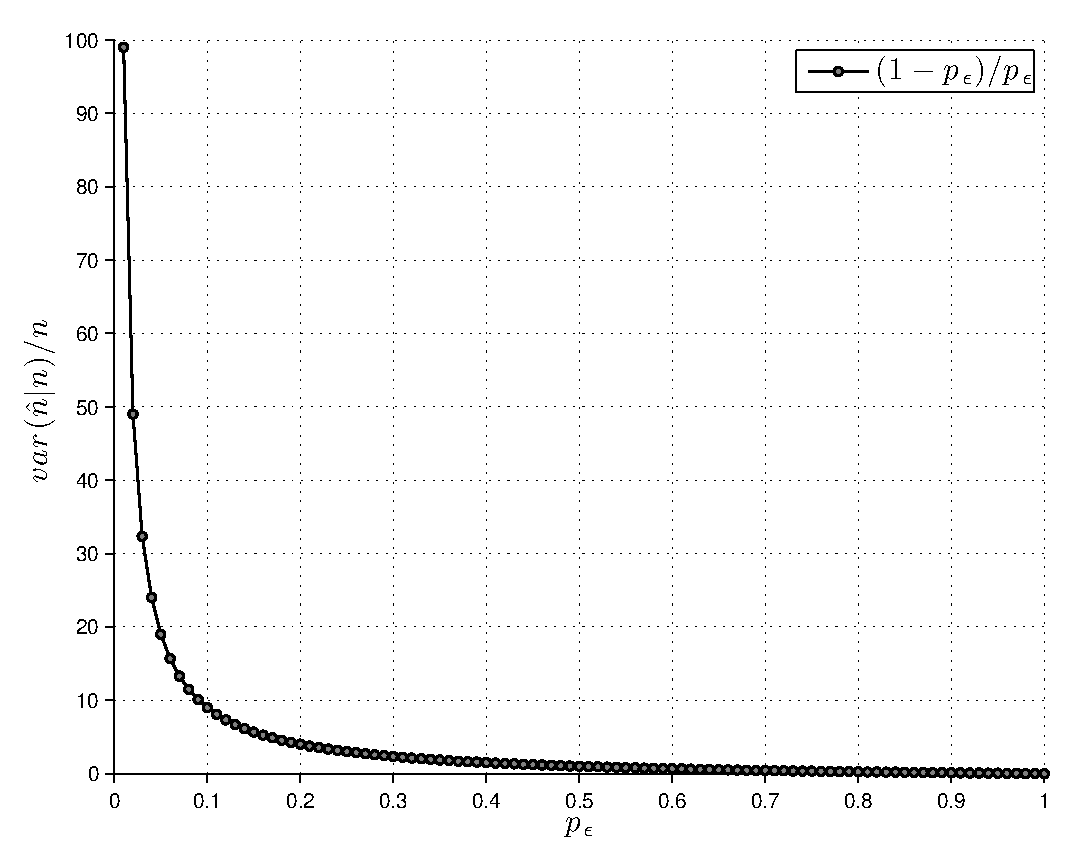
\includegraphics[scale=0.7]{matlab/Cidon/cidon-variance-p}
%\epsfile{file=matlab/Cidon/cidon-variance-p.eps,scale=0.8}
\caption[\emph{Cidon}: Variance behavior]{\emph{Cidon}:  estimate accuracy dramatically improves while $\pc\leq0.1$.}
\end{center}
\end{figure}

Variance is strict monotonically decreasing in $\pc$.
Anyway it is difficult to establish in what measure an estimate can be considered accurate.\\
Given $n$, let $k \geq1$ define the minimum required accuracy in the following way: 
\begin{equation}
\frac{n}{k}\leq\hat{n}\leq kn
\label{cidon-accuracy-constrains}
\end{equation}
Let $\theta$ be the probability we require for constrains \eqref{cidon-accuracy-constrains} to be satisfied.\\
If we set $\theta=0.99$, we can find the minimum $\pc$, ensuring the estimate to be within confidence interval \eqref{cidon-accuracy-constrains}, by solving the following problem.\\
\begin{equation}
\begin{split}
P\left(\frac{n}{k}\leq \hat{n} \leq kn \big| k,n\right)=& P\left(\frac{n}{k}\leq j/\pc \leq kn \big| k,n,\pc\right)\\
=&P\left(\frac{n\pc}{k}\leq j \leq kn\pc \big| k,n,\pc\right)
\end{split}
\label{cidon-accuracy-bounds}
\end{equation}
Probability in \eqref{cidon-accuracy-bounds} is well behaved and expresses a constrain for $j$, which is a value assumed by $J$ mentioned in \eqref{cidon-J}. Since $J$ assumes positive integer values we introduce rounding operations. In particular, rounding effect is non neglectible when $n\leq 200$.  \\
\begin{equation}
f(k,n,\pc) = P\left(\left\lceil \frac{n\pc}{k}\right\rceil\leq j \leq \left\lfloor kn\pc\right\rfloor \big| k,n,\pc\right)\geq \theta
\end{equation}
Fixed $k$, $n$ and $\theta$, $\pc$ can be found by numerically solving\footnote{in this work we used bisection method}:
\begin{equation}
f(k,n,\pc) = \theta
\end{equation}
Figure below shows $\pc$ in function of $k$ for different batch sizes.\\

\begin{figure}[htbp]
\begin{center}
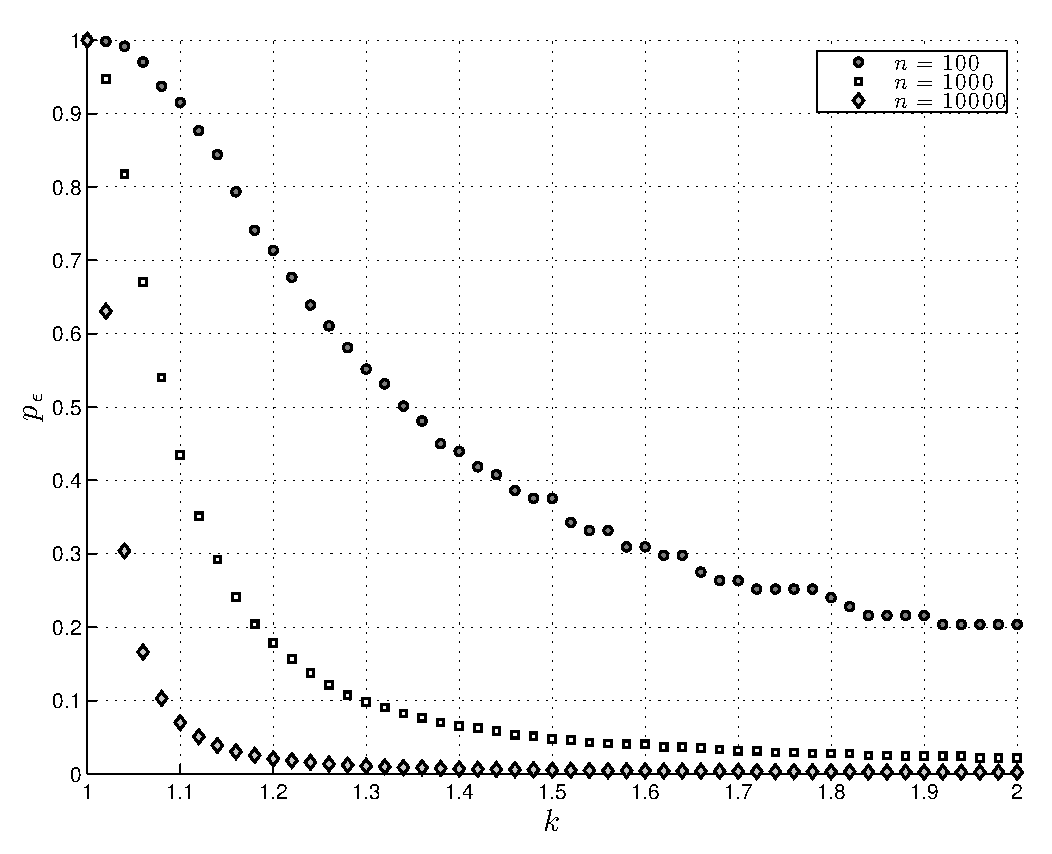
\includegraphics[scale=0.7]{matlab/Cidon/cidon-k-p-minimum}
\caption[\emph{Cidon}: Minimum $\pc$ required for accuracy $k$]{\emph{Cidon}: Minimum $\pc$ required for accuracy $k$ with $\theta=0.99$. $k$ step is 0.02}
\label{cidon-k-p-minimum}
\end{center}
\end{figure}

Figure \ref{cidon-k-p-minimum} shows how the fraction of the initial batch to resolve for estimate to be within  required confidence interval with high probability deeply depends on the size of the problem: smaller sizes require much higher $\pc$.\\
At the same time, considering absolute cost in elapsed slots, Figure  \ref{cidon-k-L-minimum} shows that, for a wide range of $k$, the time required is quite independent of the size of the problem.\\
Time required by the largest considered $n$ provides a  bound for smaller ones.\\
Note that in Figure  \ref{cidon-k-L-minimum} an upper bound on the expected BRI time taken is plotted: this bound is not so tight for very small batches. With small batches BRAs performs better than what is reported.   

\begin{figure}[htb!]
\begin{center}
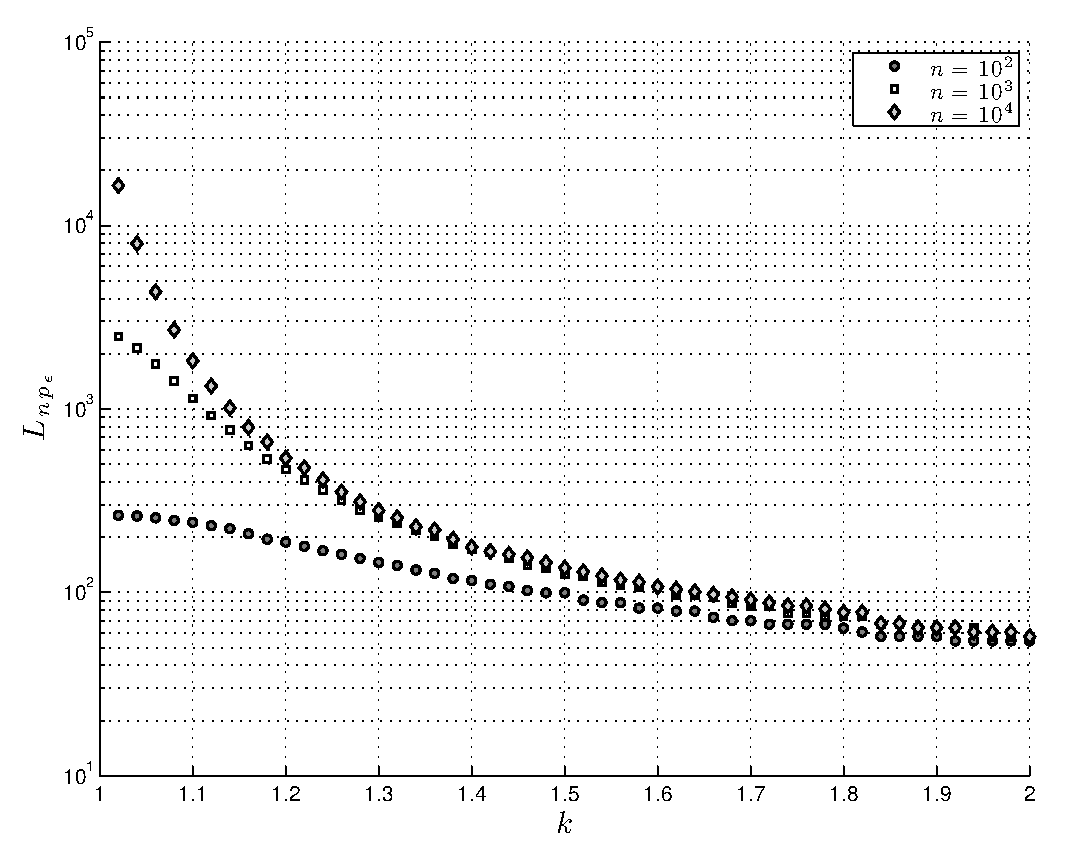
\includegraphics[scale=0.7]{matlab/Cidon/cidon-k-L-minimum}
\caption[\emph{Cidon}: Upper bounds on the expected time (in slots) required to achieve accuracy $k$]{\emph{Cidon}: Upper bounds on the expected time (in slots) required to achieve accuracy $k$ with $\theta=0.99$. $k$ step is 0.02}
\label{cidon-k-L-minimum}
\end{center}
\end{figure}

\section{Greenberg Evaluation}
Given a current slot transmission probability $p$ and a batch of size $n$ we define respectively:
\begin{enumerate}
\item the probability to get an empty slot (no transmissions)
\begin{equation}q_{0}(p,n)=(1-p)^{n} \label{eq:greenberg-prob-empty}\end{equation}
\item the probability to get a successful transmission (one transmission)
\begin{equation}q_{1}(p,n)=n p (1-p)^{n-1} \label{eq:greenberg-prob-succ}\end{equation} 
\item the probability to get a collision (two or more transmissions)
\begin{equation}q_{2+}(p,n)=1-q_{0}(p,n)-q_{1}(p,n)\label{eq:greenberg-prob-coll}\end{equation}
\end{enumerate}

In basic Greenberg (\emph{Alg.} \ref{alg-greenberg}) each slot is associated with a different probability p. Naming each slot $i$ starting with 1, 2, \dots, we have:
\begin{equation}
	p_{i}=p(i)=2^{i}
\end{equation}

Given $n$ nodes, the probability to terminate algorithm \ref{alg-greenberg} in slot $i$ is given by:
\begin{equation}
f(n,i)=\prod_{k=1}^{i-1}q_{2+}(p_{k},n) \cdot \bigl( q_{0}(p_{i},n)+q_{1}(p_{i},n)\bigr)  
\label{eq:bgstopprobability}
\end{equation}

An overview of the behavior of $f(n,i)$ is presented in table \ref{basic-greenberg-stop-probabilities} on page \pageref{basic-greenberg-stop-probabilities}.\\
\begin{equation}
\textrm{Pr}\left( \hat{n}=2^{i}|n\right)=f(n,i)  
\end{equation}

Following Figures \ref{fig:greenberg-dist-small} and \ref{fig:greenberg-dist-large} show how the distribution behave for small and large sizes.
We note that, for any fixed $n$, the distribution is well behaved: initially it is monotonically increasing, then a monotonically decreasing part follows.\\
It turns out that, for batch sizes larger than 128, the distribution is ``stable'' in the sense that doubling the number of nodes produces a shift of 1 slot to the right but the values assumed are the same (see Figure \ref{fig:greenberg-dist-large} ).\\


\begin{figure}[htbp]
\begin{center}
%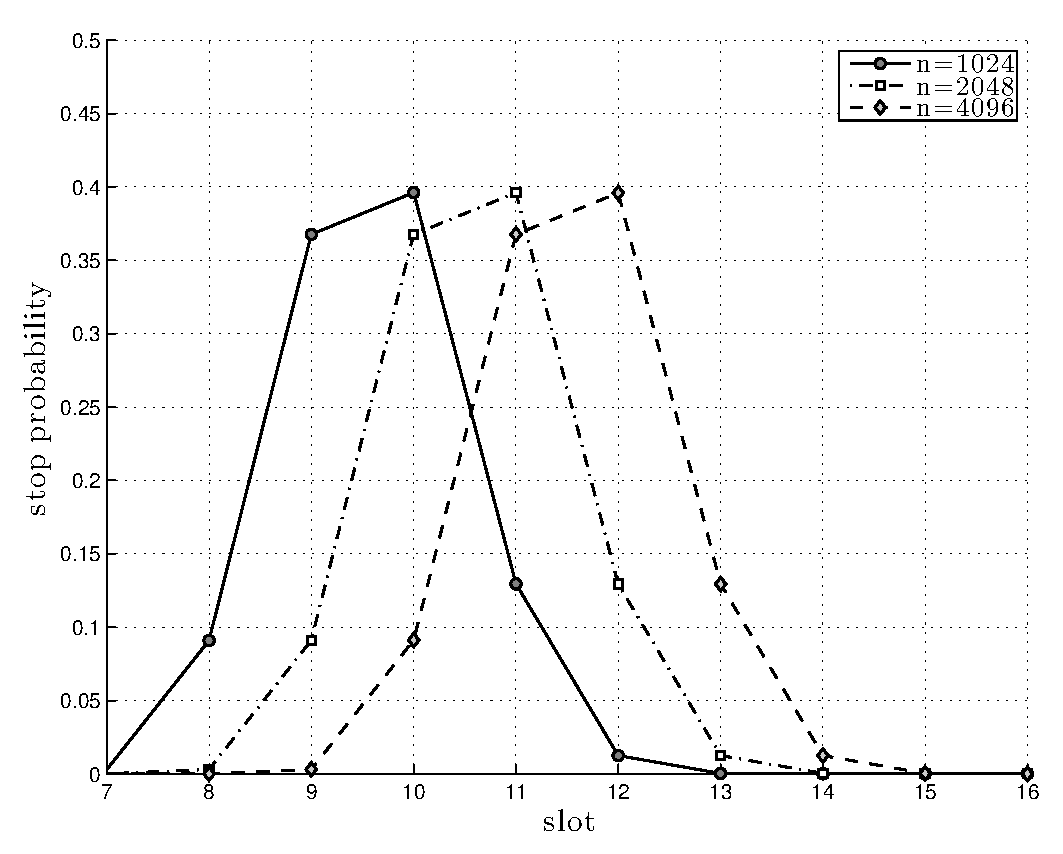
\epsfig{file=matlab/Greenberg_stop_prob/greenberg-stop-distribution-uniformity.eps,scale=0.7}
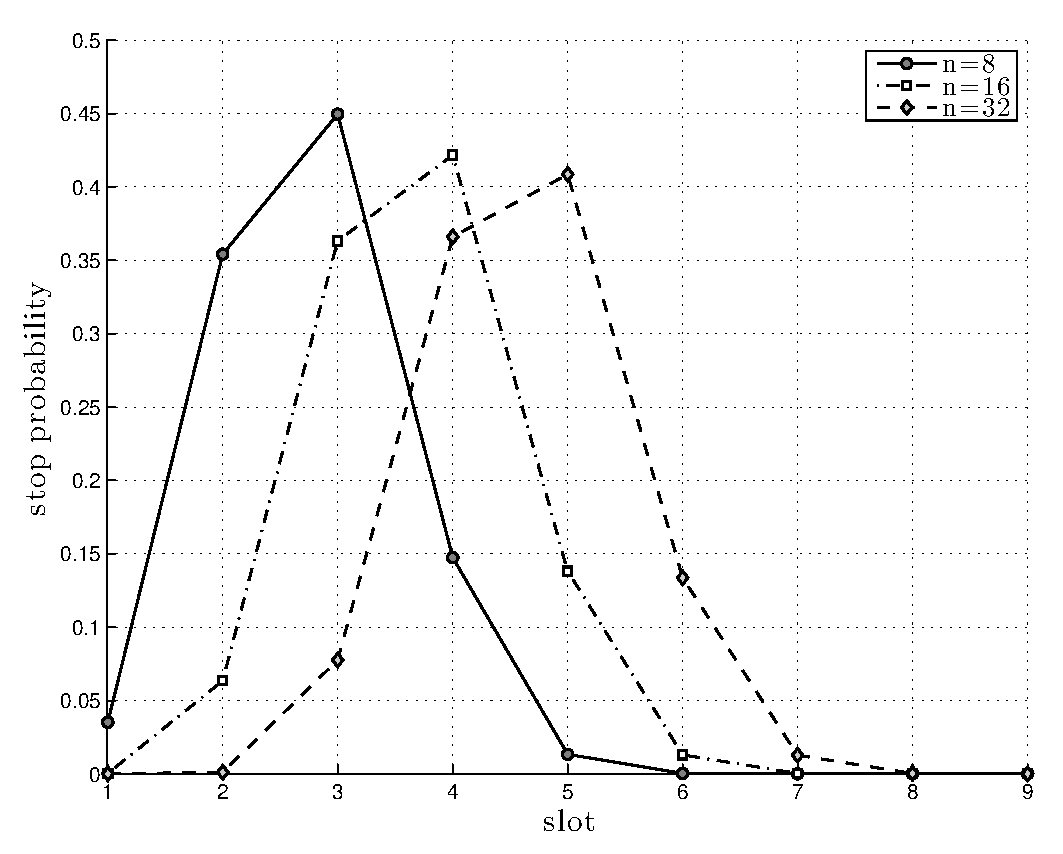
\includegraphics[scale=0.7]{matlab/Greenberg_stop_prob/greenberg-stop-distribution-uniformity-init}
\caption{\emph{Basic Greenberg}:  small $2^{k}$ sizes distribution.}
\label{fig:greenberg-dist-small}
\end{center}
\end{figure}


\begin{figure}[H]
\begin{center}
%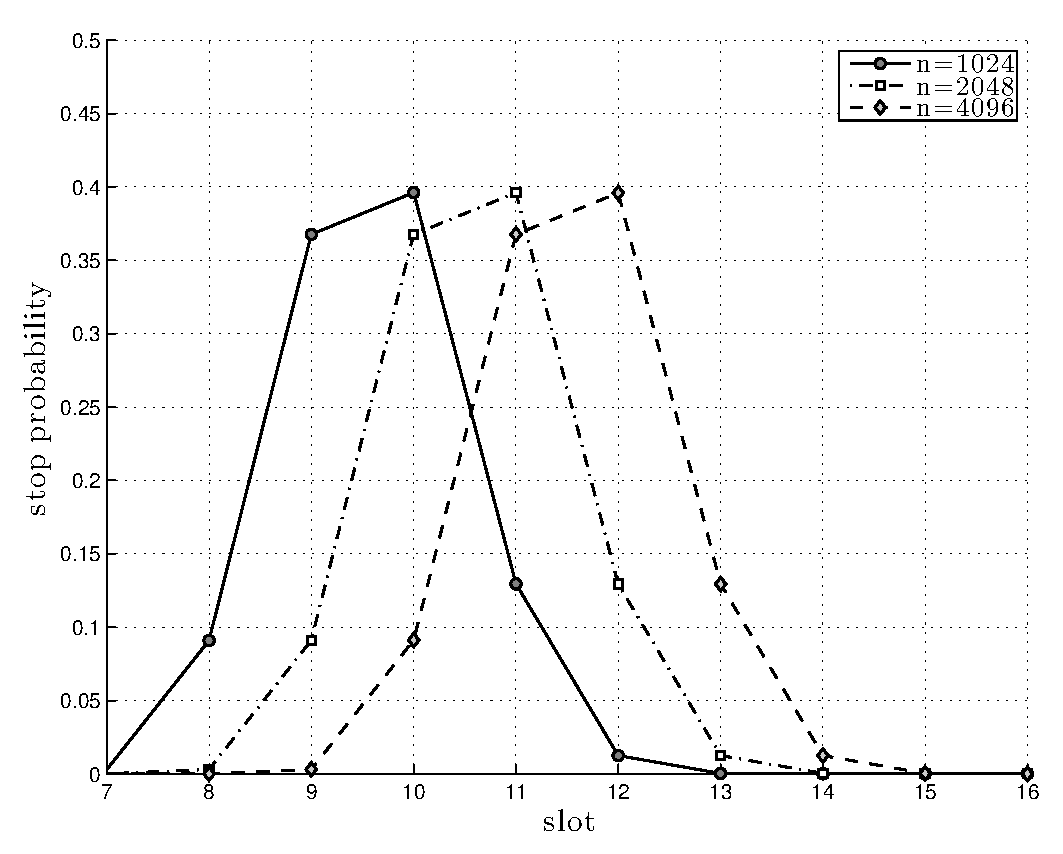
\epsfig{file=matlab/Greenberg_stop_prob/greenberg-stop-distribution-uniformity.eps,scale=0.7}
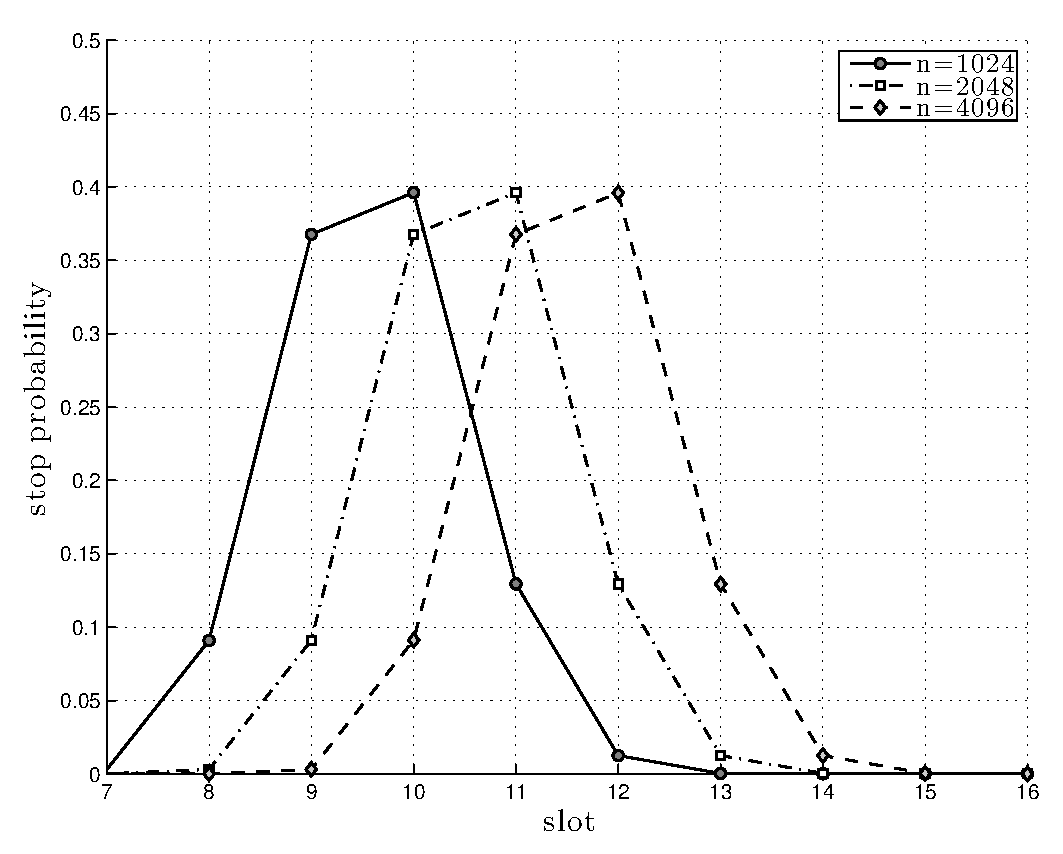
\includegraphics[scale=0.7]{matlab/Greenberg_stop_prob/greenberg-stop-distribution-uniformity}
\caption{\emph{Basic Greenberg}:  large $2^{k}$ sizes distribution.}
\label{fig:greenberg-dist-large}
\end{center}
\end{figure}


\begin{figure}[H]
\begin{center}
%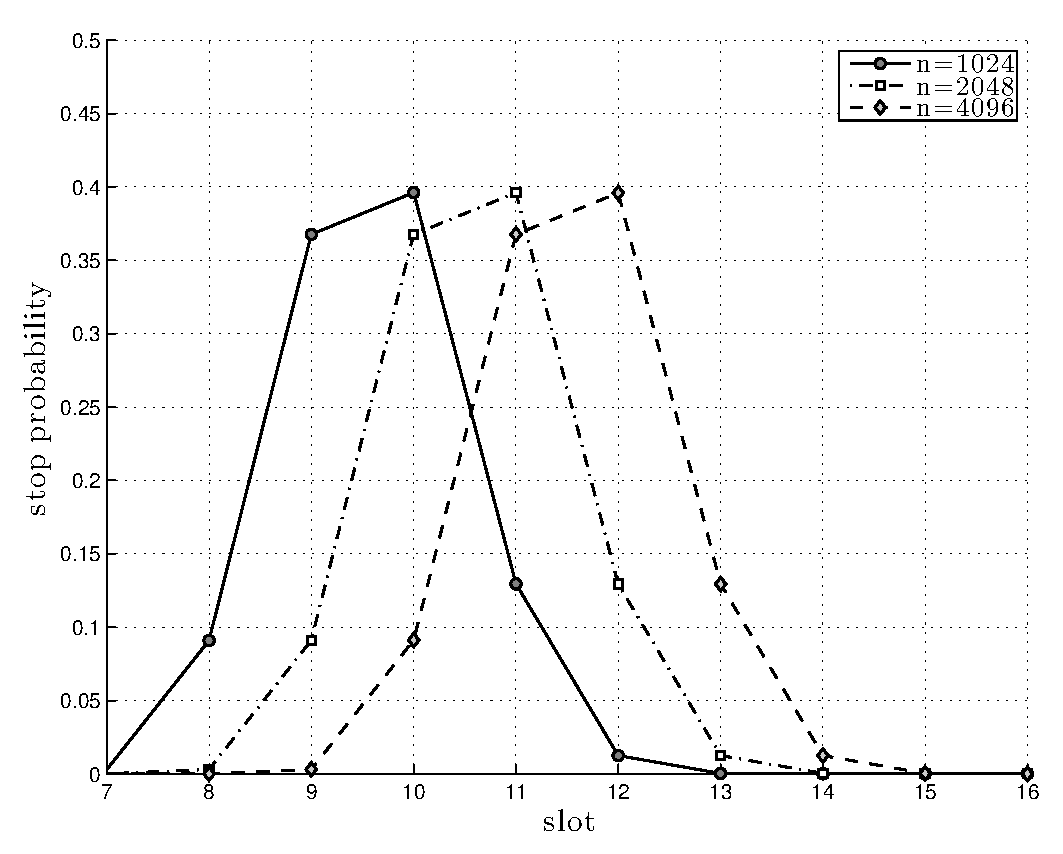
\epsfig{file=matlab/Greenberg_stop_prob/greenberg-stop-distribution-uniformity.eps,scale=0.7}
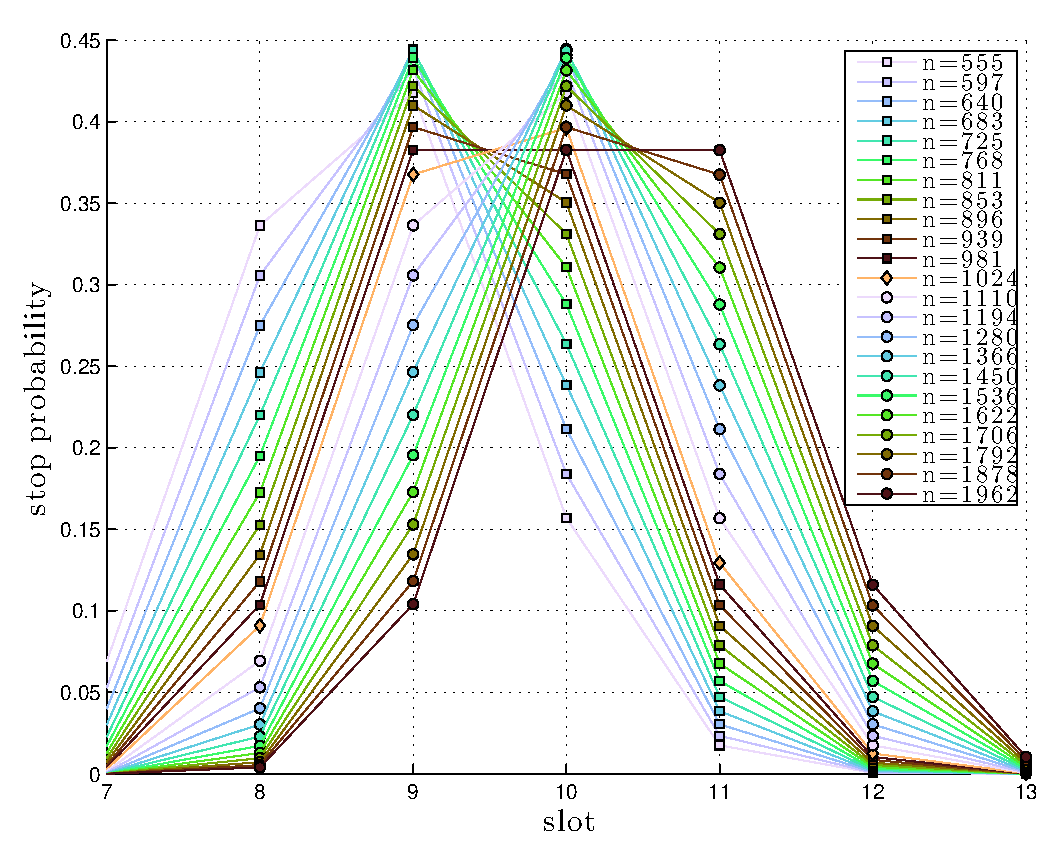
\includegraphics[scale=.7]{matlab/Greenberg_stop_prob/greenberg-stop-distribution-intermediate-values}
\caption{\emph{Basic Greenberg}:  general sizes distribution.}
\label{fig:greenberg-dist-general}
\end{center}
\end{figure}
This is not only true for sizes power of two but for any size. Figure \ref{fig:greenberg-dist-general} shows the case where size $n'$ has color $c$ and size $2n'$ has, again, color $c$ but a different marker: values are the same but shifted right. Interestingly the highest peaks are located in $n=683$ and $n=1366$.

\subsection{base $b$ Greenberg}
\subsection{Considerations}
Greenberg method is really good from the point view of running cost since it is $O\bigl(\log_{2}n\bigr)$ respect to the size  $n$ of the problem but it has also some non negligible drawbacks:
\begin{enumerate}[\bf a)]
\item estimation phase results in a sequence of colliding messages. These provides informations about the cardinality of the batch but do not help to solve an, even small, portion of the eventually following batch resolution problem and can not carry auxiliary infromations. An algorithm that allows to get an estimate while transmitting successfully messages would offer some advantages when the problem is not only the pure estimation but also a subsequent resolution.
\item it does not allow to achieve arbitrary precision in the estimate.\\ In fact we have that:
	\begin{enumerate}[\it i.]
		\item  the estimate is, by construction, a power of 2. Only a small subset of batch sizes can be mapped without any error.
		\item the end-up distribution is not sharp enough but it spans over a few slots: this is shown by Figure \ref{fig:greenberg-dist-large}. The Figure shows that, for the examined batch sizes, fixed a problem of size $n$ we have about:
		\begin{itemize}
		\item 0.02\textpertenthousand\  estimate is $16n$;
		\item 3\textpertenthousand\  estimate is $8n$;
		\item 1.2\% estimate is $4n$;
		\item 12.9\% estimate is $2n$;
		\item 39.6\% estimate is $n$; $\checkmark$
		\item 36.8\% estimate is $\frac{n}{2}$;
		\item \ 9.1\% estimate is $\frac{n}{4}$;
		\item \  3 \textperthousand\ estimate is $\frac{n}{8}$;
		\item \ 0.02\textpertenthousand\ estimate is $\frac{n}{16}$;
		\end{itemize}
		It is difficult to discriminate between $n$ and $\frac{n}{2}$ 
	\end{enumerate}
\item to get a tighter estimate, base $b$ Greenberg has to be used. Anyway to improve the accuracy very small $b$ has to be used (see Table \ref{table:greenberg-b-phi}) and this results in a worse running times: even if theoretically it remains $O(log_{b}n)$ which is a lower order term compared to $n$, in practice estimate time can be no more neglected. In this case, for reasons expressed in {\bf a)}, using Greenberg  could be a bad choice.
\end{enumerate}

\section{Greenberg with MLE}

Let $n$ be a batch size and $p$ be a given transmission probability. As expressed by \eqref{eq:greenberg-prob-empty} \eqref{eq:greenberg-prob-succ} \eqref{eq:greenberg-prob-coll}, varying $n$ while $p$ is fixed results in very different probabilities for \emph{idle}, \emph{successful} and \emph{collided} slots.

\begin{figure}[H]
\begin{center}
%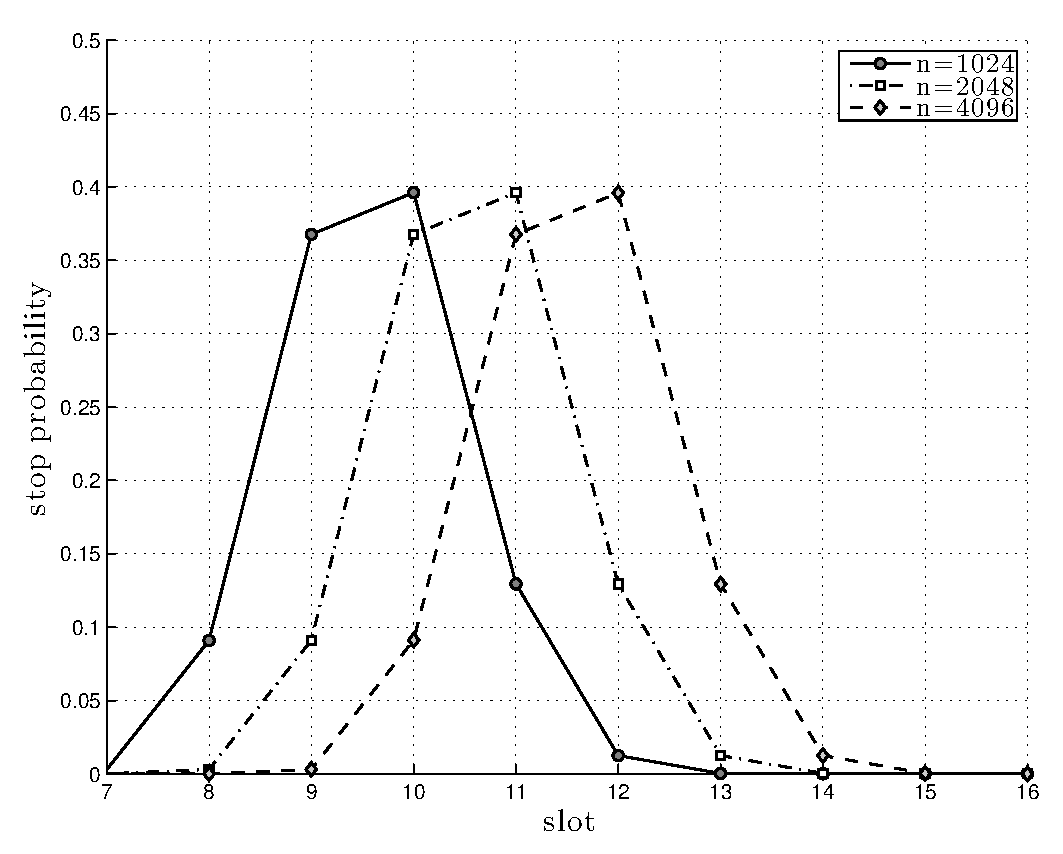
\epsfig{file=matlab/Greenberg_stop_prob/greenberg-stop-distribution-uniformity.eps,scale=0.7}
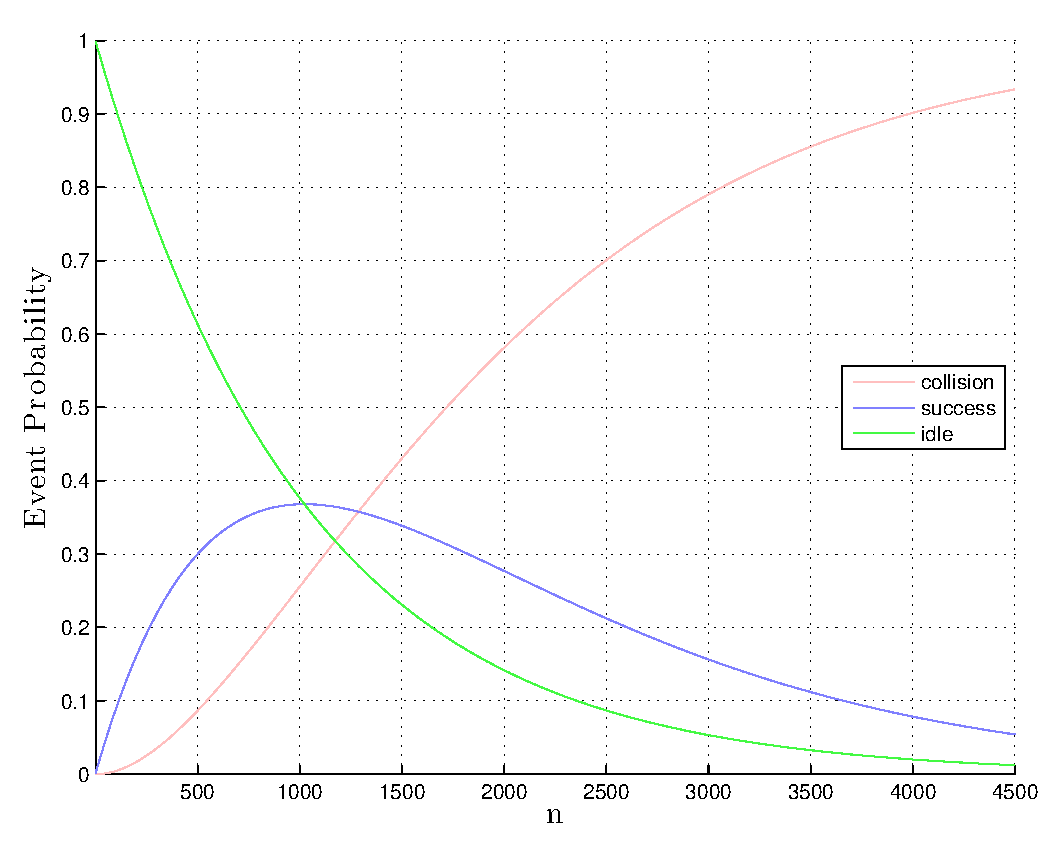
\includegraphics[scale=.7]{matlab/Greenberg_MLE/draw_coll_idle_succ_fixed_p}
\caption[Event probability fixed $p$]{Event probability for fixed $p=1/1024$.  $q_{0}(p,n) \approx  q_{1}(p,n)$ for $n=1023$}
\end{center}
\end{figure}

It is quite immediate to see that:
\begin{itemize}
\item $q_{0}(p,n) \approx q_{1}(p,n)$ when $n\approx 1/p$ and, obviously,
\item $q_{0}(p,n) \gg q_{1}(p,n)$ and $q_{0}(p,n) \gg q_{2+}(p,n)$ when $n \ll 1/p$
\item $q_{2+}(p,n) \gg q_{0}(p,n)$ and $q_{2+}(p,n) \gg q_{0}(p,n)$ when $n \gg 1/p$
\end{itemize}
$q_{2+}(p,n)$ is strictly increasing monotonic while $q_{0}(p,n)$ is strictly decreasing. If we could repeat a large number $T$ of test transmission with  probability $p$ each, we could simply use the ratio collision/$T$ or idle/$T$ to uniquely determined our batch size. This is not true for successful transmissions since $q_{1}(p,n)$ is non-monotonic.\\
 
 Let $T$ be a number of slots of our choice and $N_{0}$, $N_{1}$, $N_{2+}$ random variables which represent the number of time slots with no transmissions, one transmission and collision respectively.\\
 sono binomiali\\
 Of course $N_{0}+N_{1}+N_{2+}=T$ and
 \begin{eqnarray*}
E[N_{0}] &=& Tq_{0}(p,n)\\
E[N_{1}] &=& Tq_{1}(p,n)\\
E[N_{2+}] &=& Tq_{2+}(p,n)
\end{eqnarray*}


\begin{equation}
f_{T}(i,s,c,p',n')= \textrm{Pr}(N_{0}=i,N_{1}=s,N_{2+}=c|n=n',p=p')
\end{equation}

\begin{equation}
MLE(i,s,c,l)=\argmax_{\displaystyle{n'}} \Bigl( f_{T}\bigl(i,s,c,p(l),n')\cdot f\bigl(n',l\bigr)\Bigr)
\end{equation}

\chapter{Comparison}
\label{ch:Comparison}







\begin{comment}

\begin{sidewaystable}
\centering
\begin{tabular}{|llllllllp{1in}lp{1in}|}
\hline
Context   &Length   &Breadth/   &Depth   &Profile   &Pottery   &Flint   &Animal   &Stone   &Other    &C14 Dates \\
  &         &Diameter   &        &          &          &        & 
Bones&&&\\
\hline
&&&&&&&&&&\\
\multicolumn{10}{|l}{\bf Grooved Ware}&\\
784 &---   &0.90m &0.18m &Sloping U &P1    &$\times$46  &  $\times$8  &&$\times$2 bone&  2150$\pm$ 100 BC\\
785 &---   &1.00m &0.12  &Sloping U &P2--4 &$\times$23  &  $\times$21 & Hammerstone &---&---\\
962 &---   &1.37m &0.20m &Sloping U &P5--6 &$\times$48  &  $\times$57* & ---&     ---&1990 $\pm$ 80 BC (Layer 4) 1870 $\pm$90 BC (Layer 1)\\
983 &0.83m &0.73m &0.25m &Stepped U &---   &$\times$18  &  $\times$8 & ---& Fired clay&---\\
&&&&&&&&&&\\
\multicolumn{10}{|l}{\bf Beaker}&\\
552 &---   &0.68m &0.12m &Saucer    &P7--14 &---        & --- & --- &--- &---\\
790 &---   &0.60m &0.25m &U         &P15    &$\times$12 & --- & Quartzite-lump&--- &---\\
794 &2.89m &0.75m &0.25m &Irreg.    &P16    $\times$3   & --- & --- &--- &---\\
\hline
\end{tabular}
 
\caption[Grooved Ware and Beaker Features, their Finds and Radiocarbon
Dates]{Grooved Ware and Beaker Features, their Finds and Radiocarbon
Dates; For a breakdown of the Pottery Assemblages see Tables I and
III; for the Flints see Tables II and IV; for the Animal Bones see
Table V.}\label{rotfloat2} \end{sidewaystable} 
\end{comment}

\begin{appendices}

\chapter[Appendix]{}

\section{Probability}
\textcolor{red}{sezione provvisoria}
\subsection{Chebyshev's inequality}
Let $X$ be a \emph{random variable} with expected value $\mu$ and finite variance $\sigma^{2}$. Then for any real number $k>0$,
\begin{equation}
\Pr(\left|X-\mu\right|\geq k)\leq\frac{\sigma^{2}}{k^2}
\label{eq:cheby}
\end{equation}
\subsection{Binomial Distribution}

$B(n,p)$
\subsubsection{Poisson Approximation}
The binomial distribution converges towards the Poisson distribution as the number of trials goes to infinity while the product $np$ remains fixed. Therefore the Poisson distribution with parameter $\lambda = np$ can be used as an approximation to $B(n, p)$ of the binomial distribution if $n$ is sufficiently large and $p$ is sufficiently small. According to two rules of thumb, this approximation is good if $n \geq 20$ and $p \leq 0.05$, or if $n \geq 100$ and $np \leq 10$.
\subsubsection{Normal Approximation}
If $n$ is large enough, then the skew of the distribution is not too great. In this case, if a suitable continuity correction is used, then an excellent approximation to $B(n, p)$ is given by the normal distribution $\mathcal{N}(np,np(1-p))$\\
The approximation generally improves as $n$ increases and is better when $p$ is not near to 0 or 1. Various rules of thumb may be used to decide whether $n$ is large enough, and $p$ is far enough from the extremes of zero or unity:
One rule is that both $n p$ and $n(1-p)$ must be greater than 5. However, the specific number varies from source to source, and depends on how good an approximation one wants; some sources give 10.\\

oppure dal libro $np(1-p)\geq 10$.




\subsection{Poisson Distribution}
\subsection{Normal Distribution}
 $\mathcal{N}(\mu,\sigma^{2})$
\begin{equation}
f(x)= \frac{1}{\sqrt{2\pi\sigma^{2}}}\exp{-\frac{(x-\mu)^{2}}{2\sigma^{2}}}
\end{equation}

\section{Greenberg bounded \emph{m}-moments}

In general for base $b$ greenberg algorithm the first and second moments are bounded by:

\begin{equation}
\phi(b)= \frac{1}{\log b} \int_{0}^{\infty} \! e^{-x}(1+x) \prod_{k=1}^{\infty}(1-e^{-b^{k}x}(1+b^{k}x))x^{-2} \, dx
\end{equation}

\begin{equation}
\Phi(b)= \frac{1}{\log b} \int_{0}^{\infty} \! e^{-x}(1+x) \prod_{k=1}^{\infty}(1-e^{-b^{k}x}(1+b^{k}x))x^{-3} \, dx
\end{equation}

\textcolor{red}{note sul calcolo\\ va velocemente a 0 quind basta considerare un intervallo iniziale  limitato\\
anche per produttoria con k è lo stesso.\\ risolto con quad matlab}

\section{CBT Estimate Experimental Distribution}

Following tables \ref{CBT-table-1} shows the behavior of CBT Algorithm (section \ref{cbt-estimation}) for estimation.  Simulation was implemented in matlab.
The resulting distribution of $\hat{n}$ fixed $n$ is the result of averaging \numprint{100000} runs of CBT Algorihm applied on uniformly random generated nodes ID batches.\\ 

\begin{table}[H]
\caption[Experimentally computed CBT Estimate Distributon]{Experimentally computed CBT Estimate Distributon. Table 1/3}
\label{CBT-table-1}
\resizebox{\textwidth}{!}{
\begin{tabular}{r|cccccccccccc}
n&$\hat{n}:$&2&4&8&16&32&64&128&256&512&1024&2048 \\\hline

2 &&0.499 &0.253 &0.125 &0.061 &0.031 &0.015 &0.007 &0.004 &0.002 &9e-04 &4e-04\\\hline

4 &&&0.189 &0.303 &0.225 &0.133 &0.072 &0.038 &0.020 &0.010 &0.005 &0.002\\\hline

8 &&&0.055 &0.212 &0.261 &0.201 &0.126 &0.071 &0.037 &0.019 &0.009 &0.005\\\hline

16 &&&8e-04 &0.070 &0.209 &0.252 &0.197 &0.125 &0.070 &0.038 &0.019 &0.010\\\hline

32 &&&&0.003 &0.075 &0.213 &0.249 &0.195 &0.123 &0.069 &0.037 &0.018\\\hline

64 &&&&&0.004 &0.077 &0.208 &0.250 &0.193 &0.124 &0.069 &0.037\\\hline

128 &&&&&&0.005 &0.081 &0.208 &0.247 &0.191 &0.123 &0.069\\\hline

256 &&&&&&2e-05 &0.006 &0.079 &0.209 &0.246 &0.193 &0.123\\\hline

512 &&&&&&&&0.005 &0.081 &0.207 &0.245 &0.193\\\hline

1024 &&&&&&&&&0.005 &0.080 &0.208 &0.245\\\hline

2048 &&&&&&&&&2e-05 &0.005 &0.080 &0.209\\\hline

4096 &&&&&&&&&&1e-05 &0.006 &0.082\\\hline

8192 &&&&&&&&&&&1e-05 &0.006\\\hline

16384 &&&&&&&&&&&&2e-05\\\hline

32768 &&&&&&&&&&&&\\\hline

\end{tabular}
}

\end{table}
\begin{table}[H]
\ContinuedFloat
\caption[]{Experimentally computed CBT Estimate Distributon. Table 2/3}
\resizebox{\textwidth}{!}{
\begin{tabular}{r|cccccccccccc}
n&$\hat{n}:$&4096&8192&16384&32768&$2^{16}$&$2^{17}$&$2^{18}$&$2^{19}$&$2^{20}$&$2^{21}$&$2^{22}$ \\\hline

2 &&2e-04 &1e-04 &1e-04 &&&&1e-05 &&&&\\\hline

4 &&0.001 &5e-04 &3e-04 &1e-04 &6e-05 &4e-05 &&2e-05 &1e-05 &&\\\hline

8 &&0.002 &0.001 &6e-04 &3e-04 &9e-05 &8e-05 &4e-05 &1e-05 &&&\\\hline

16 &&0.005 &0.003 &0.001 &6e-04 &3e-04 &2e-04 &6e-05 &2e-05 &2e-05 &&\\\hline

32 &&0.009 &0.005 &0.003 &0.001 &6e-04 &3e-04 &1e-04 &1e-04 &6e-05 &1e-05 &1e-05\\\hline

64 &&0.019 &0.009 &0.005 &0.002 &0.001 &7e-04 &3e-04 &7e-05 &4e-05 &&2e-05\\\hline

128 &&0.037 &0.019 &0.010 &0.005 &0.003 &0.001 &5e-04 &4e-04 &2e-04 &5e-05 &4e-05\\\hline

256 &&0.068 &0.038 &0.019 &0.009 &0.005 &0.002 &0.001 &6e-04 &3e-04 &6e-05 &8e-05\\\hline

512 &&0.123 &0.071 &0.037 &0.019 &0.010 &0.005 &0.002 &0.001 &6e-04 &3e-04 &2e-04\\\hline

1024 &&0.193 &0.122 &0.070 &0.037 &0.019 &0.010 &0.005 &0.002 &0.001 &6e-04 &2e-04\\\hline

2048 &&0.246 &0.194 &0.123 &0.068 &0.037 &0.019 &0.010 &0.005 &0.002 &0.001 &6e-04\\\hline

4096 &&0.210 &0.246 &0.193 &0.121 &0.068 &0.037 &0.019 &0.009 &0.004 &0.003 &0.001\\\hline

8192 &&0.080 &0.208 &0.247 &0.192 &0.123 &0.070 &0.037 &0.019 &0.009 &0.005 &0.002\\\hline

16384 &&0.006 &0.080 &0.208 &0.247 &0.192 &0.123 &0.069 &0.037 &0.019 &0.010 &0.005\\\hline

32768 &&&0.006 &0.079 &0.209 &0.248 &0.194 &0.122 &0.069 &0.036 &0.019 &0.010\\\hline

\end{tabular}
}

\end{table}
\begin{table}[H]\ContinuedFloat
\caption[]{Experimentally computed CBT Estimate Distributon. Table 3/3}
\resizebox{\textwidth}{!}{
\begin{tabular}{r|ccccccccccc}
n&$\hat{n}:$&$2^{23}$&$2^{24}$&$2^{25}$&$2^{26}$&$2^{27}$&$2^{28}$&$2^{29}$&$2^{30}$&$2^{31}$&$2^{32}$ \\\hline

2 &&&&&&&&&&&\\\hline

4 &&&&&&&&&&&\\\hline

8 &&&&&&&&&&&\\\hline

16 &&&&&&&&&&&\\\hline

32 &&1e-05 &&&&&&&&&\\\hline

64 &&2e-05 &&&&1e-05 &&&&&\\\hline

128 &&4e-05 &&1e-05 &&&&&&&\\\hline

256 &&4e-05 &1e-05 &&2e-05 &&&1e-05 &&&\\\hline

512 &&7e-05 &2e-05 &1e-05 &3e-05 &1e-05 &&&&&\\\hline

1024 &&2e-04 &1e-04 &4e-05 &&2e-05 &1e-05 &&&&\\\hline

2048 &&3e-04 &1e-04 &3e-05 &3e-05 &3e-05 &3e-05 &&&&\\\hline

4096 &&6e-04 &3e-04 &9e-05 &7e-05 &1e-05 &&&&&\\\hline

8192 &&0.001 &8e-04 &3e-04 &2e-04 &8e-05 &7e-05 &2e-05 &3e-05 &1e-05 &\\\hline

16384 &&0.002 &0.001 &6e-04 &3e-04 &1e-04 &1e-04 &4e-05 &&&\\\hline

32768 &&0.005 &0.002 &0.001 &6e-04 &3e-04 &2e-04 &1e-04 &1e-05 &2e-05 &1e-05\\\hline

\end{tabular}
}
\end{table}

\lstinputlisting{matlab/CBT/cbtsimpletest.m}
\lstinputlisting{matlab/CBT/cbtsplit.m}
\lstinputlisting{matlab/CBT/cbtfulltest.m}
%\verbatiminput{matlab/CBT/cbtfulltest.m}

\section{Greenberg Estimate Distribution}
In following table \ref{basic-greenberg-stop-probabilities} we report how the end  up probability (equation \ref{eq:bgstopprobability}) is distributed among slots given a batch of size $n$.  Column ``$n$'' lists  the considered batch sizes. $\hat{n}$ is the resulting estimation (without corrections) when ending up in the underneath slot.\\  For sake of simplicity considered values are all powers of 2.\\
Datas presented were post-processed to become more accessible:
\begin{itemize}
\item values above $10^{-3}$ are reported in format ('\emph{\%1.3f}');
\item values below $10^{-12}$ are not presented since are tight close to 0.
\item other values are presented in exponential notation and rounded to the first meaningful digit ('\emph{\%1.e}')
\end{itemize}


\begin{sidewaystable}
%%%%%
\flushleft
\resizebox{25cm}{!}{
\begin{tabular}{r|ccccccccccccccccccccccc}
&$\hat{n}$& 2 &4 &8 &16 &32 &64 &128 &256 &512 &1024 &2048 &4096 &8192 &16384 &32768 &65536\\
n & slot:& 1 &2 &3 &4 &5 &6 &7 &8 &9 &10 &11 &12 &13 &14 &15 & 16\\ 
\toprule
1 &&1.000 &&&&&&&&&\\\hline

2 &&0.750 &0.234 &0.015 &2e-04 &1e-06 &9e-10 &&&&&&&&\\\hline

4 &&0.312 &0.508 &0.166 &0.014 &3e-04 &2e-06 &2e-09 &&&&&&&\\\hline

8 &&0.035 &0.354 &0.450 &0.147 &0.013 &3e-04 &2e-06 &4e-09 &1e-12 &&&&&&\\\hline

16 &&3e-04 &0.063 &0.363 &0.422 &0.138 &0.013 &3e-04 &2e-06 &4e-09 &2e-12 &&&&&\\\hline

32 &&8e-09 &0.001 &0.078 &0.366 &0.409 &0.134 &0.013 &3e-04 &2e-06 &4e-09 &2e-12 &&&&\\\hline

64 &&&2e-07 &0.002 &0.084 &0.367 &0.402 &0.131 &0.013 &3e-04 &2e-06 &4e-09 &2e-12 &&&\\\hline

128 &&&&7e-07 &0.002 &0.088 &0.367 &0.399 &0.130 &0.013 &3e-04 &2e-06 &5e-09 &2e-12 &&\\\hline

256 &&&&&1e-06 &0.003 &0.090 &0.368 &0.397 &0.130 &0.013 &3e-04 &2e-06 &5e-09 &2e-12 & \\\hline

512 &&&&&&2e-06 &0.003 &0.090 &0.368 &0.397 &0.130 &0.012 &3e-04 &2e-06 &5e-09 &2e-12 \\\hline
1024 &&&&&&&2e-06 &0.003 &0.091 &0.368 &0.396 &0.129 &0.012 &3e-04 &2e-06 &5e-09 &2e-12 \\
\bottomrule
\end{tabular}
}

\begin{tabular}{c}
\\
\end{tabular}
\resizebox{25cm}{!}{
\begin{tabular}{r|ccccccccccccccccccccccc}
&$\hat{n}$&128 &256 &512 &1024 &2048 &4096 &8192 &16384 &32768 &65536 &$2^{17}$ &$2^{18}$ &$2^{19}$ &$2^{20}$ &$2^{21}$ &$2^{22}$ \\ 
n & slot:& 7 &8 &9 &10 &11 &12 &13 &14 &15 &16 &17 &18 &19 &20 &21 &22 \\ 
\toprule


2048 &&2e-06 &0.003 &0.091 &0.368 &0.396 &0.129 &0.012 &3e-04 &2e-06 &5e-09 &2e-12 &&&&&\\\hline

4096 &&&2e-06 &0.003 &0.091 &0.368 &0.396 &0.129 &0.012 &3e-04 &2e-06 &5e-09 &2e-12 &&&&\\\hline

8192 &&&&2e-06 &0.003 &0.091 &0.368 &0.396 &0.129 &0.012 &3e-04 &2e-06 &5e-09 &2e-12 &&&\\\hline

16384 &&&&&2e-06 &0.003 &0.091 &0.368 &0.396 &0.129 &0.012 &3e-04 &2e-06 &5e-09 &2e-12 &&\\\hline

32768 &&&&&&2e-06 &0.003 &0.091 &0.368 &0.396 &0.129 &0.012 &3e-04 &2e-06 &5e-09 &2e-12 &\\\hline

65536 &&&&&&&2e-06 &0.003 &0.091 &0.368 &0.396 &0.129 &0.012 &3e-04 &2e-06 &5e-09 &2e-12\\

\bottomrule
\end{tabular}
}
%%%%
\caption{Analytically computed basic Greeenberg Estimate Distribution}
\label{basic-greenberg-stop-probabilities}

\end{sidewaystable}

\end{appendices}


\begin{thebibliography}{99}
 
\bibitem{popovski}
  Peter Popovski, Frank H.P. Fitzek, Ramjee Prasad, \emph{ A Class of Algorithms for Collision Resolution with Multiplicity Estimation}, Springer, Algorithmica, Vol. 49, No. 4, December 2007, 286-317
  
\bibitem{lucent}
Murali Kodialam, Thyaga Nandagopal, \emph{Fast and Reliable Estimation Schemes in RFID Systems}, MobiCom '06: Proceedings of the 12th annual international conference on Mobile computing and networking, ACM , September 2006, 322-333 
 
\bibitem{cidon}
 Israel Cidon, Moshe Side, \emph{Conflict Multiplicity Estimation and Batch Resolution Algorithms}, IEEE Transactions On Information Theory, Vol. 34, No. 1, January 1988, 101-110
 
\bibitem{greenberg87}
  Albert G. Greenberg, Philippe Flajolet,  Richard E. Ladner,
  \emph{Estimating the Multiplicities of Conflicts to Speed Their Resolution in Multiple Access Channels},
  Journal of the Association for Computing Machinery,
  Vol 34, No. 2, April 1987, 289-325
  
 \bibitem{capetanakis}
  J.I. Capetanakis, \emph{ Tree algorithms for packet broadcast channels}, IEEE Transactions On Information Theory, Vol. 25, No. 5, September 1979, 505-515
 \end{thebibliography}
\end{document}